\documentclass[10pt]{report}
\usepackage{amsmath, amsthm, amssymb, tikz, mathtools, hyperref, enumerate}
\usepackage[margin=0.5in]{geometry}
\newcommand{\scinot}[2]{#1\times 10^{#2}}
\newcommand{\bra}[1]{\left<#1\right|}
\newcommand{\ket}[1]{\left|#1\right>}
\newcommand{\dotp}[2]{\left<#1\left.\right|#2\right>}
\newcommand{\rd}[2]{\frac{d#1}{d#2}}
\newcommand{\pd}[2]{\frac{\partial #1}{\partial#2}}
\newcommand{\norm}[1]{\left|\left|#1\right|\right|}
\newcommand{\abs}[1]{\left|#1\right|}
\newcommand{\expvalue}[1]{\left<#1\right>}
\newcommand{\rtd}[2]{\frac{d^2#1}{d#2^2}}
\newcommand{\pvec}[1]{\vec{#1}^{\,\prime}}
\let\Re\undefined
\let\Im\undefined
\DeclareMathOperator{\Re}{Re}
\DeclareMathOperator{\Tr}{Tr}
\DeclareMathOperator{\Im}{Im}
\newcommand{\ptd}[2]{\frac{\partial^2 #1}{\partial#2^2}}
\usepackage[labelfont=bf, font=scriptsize]{caption}
\everymath{\displaystyle}

\begin{document}

\title{Quantum solid-state physics: an introduction\\ Amphi Poisson W 0830-1000, 1330-1500\\ Antoine Georges CPHT-X}
\author{Yubo Su}
\date{}

\maketitle
\tableofcontents

\chapter{10/09/14 --- Overview of condensed matter}

Both lectures and PCs will be in English (thank God) to cater to the international audience. Website can be found by googling PHY552A. Emails are
\begin{itemize}
    \item Antoine Georges (lecturer) --- antoine.georges@polytechnique.edu
    \item Michel Ferrero (PC) --- michel.ferrero@polytechnique.edu
    \item Edward Perepelitsky --- edward.perepelitsky@polytechnique.edu
\end{itemize}

\textbf{Homework assignments:} multiple choice questions (about 20 minutes) at \url{http://www.enseignement.polytechnique.fr/profs/physique/Manuel.Joffre/qcm}. Login just uses email address. If problem logging in, manuel.joffre@polytechnique.edu, otherwise email Edward. Optional problems but highly recommended; note that participation will be taken into account for class grade.

Prerequisites include basic quantum mechanics (SE, spin, particle in a box, HO, hydrogen atom) and basic statmech (including Boltzmann/Fermi-Dirac statistics, basic properties of fermion gases). \\[10pt]

We now begin a general survey  of condensed matter physics and materials. Condensed matter physics relates macroscopic properties to microscopic calculations, spanning many orders of magnitude. A useful OoM calculation is given by $300\mathrm{K} \sim \frac{1}{40}\mathrm{eV}$. The states of matter we can study with condensed matter include
\begin{itemize}
    \item Crystals (we will handle perfect ones, but in reality they are imperfect)
    \item Amorphous solids (glass, atoms occupy disordered positions)
    \item Liquids
    \item Gases
    \item ``Soft matter'' --- between liquids/gases: gels, foams, etc.
\end{itemize}

Let's begin by discussing the Carbon atom. Its electronic configuration is 1s$^2$ 2s$^2$ 2p$^2$, so it has $4$ valence electrons, two tucked in more deeply. This organizes itself into many crystalline structures, including diamond, graphite, buckminsterfullerenes, nanotubes, glass, etc. We are curious in this class to discover why different organizations of the same atom can produce so many different properties. We can also study superconductors, which are again super-duper useful in life.

The fundamental Hamiltonian we will be studying will be some special case of the following Hamiltonian
\begin{align}
    H &= \frac{1}{2M}\sum\limits_{i=1}^{N_0}\mathbf{P}_i^2 + \frac{1}{2m_0}\sum\limits_{j=1}^{N_e}\mathbf{p}_i^2 + \frac{Z^2}{2}\sum\limits_{i,j=1, i \neq j}^{N_n} V_c(\mathbf{R}_i - \mathbf{R}_j) - Z\sum\limits_{i=1}^{N_n}\sum\limits_{j=1}^{N_e}V_c(\mathbf{r}_j - \mathbf{R}_i) + \frac{1}{2}\sum\limits_{i,j = 1, i \neq j}^{N_e}V_c(\mathbf{r}_i - \mathbf{r}_j)
\end{align}

Big letters are nucleus, little letters are the various electrons. We can of course make the simplifying assumption that nuclei are fixed, which drops the first and third terms (constant). While then the second and fourth term form a very simple Hamiltonian (separable into each of $N_e$ degrees of freedom), the fifth term (pairwise electron interactions) proves to be a big problem, an insoluble one at that. The class will then be much of approximate methods, more practical for our problems of choice. 

Let's go a bit more quantitative. In order to do this, we will first neglect the pairwise coupling of the electrons and then assume the nuclei to be immobile. This then gives the Hamiltonian
\begin{align}
    \hat{H} &= \sum\limits_{i=1}^{N_e}\hat{h}(\vec{r}_i, \vec{p}_i) \\
    \hat{h}(\vec{r},\vec{p}) &= \frac{\vec{p}^2}{2m_e} + V(\vec{r})\\
    V(\vec{r}) &= \sum\limits_{n=1}^{N}\frac{e^2}{4\pi\epsilon_0\abs{\vec{r} - \vec{R}_n}}
\end{align}

Let's first go to 1D. Now if we assume that $\vec{R}_n$ are fully periodic, such as if $R_n = na$, then the potential itself is periodic $V(x + na) = V(x)$ and so we have to solve the $1$-particle SE in a periodic potential. We will visit this problem in depth over the course of the next few lectures.

We can first examine $N=1$, the hydrogen atom, with only one electron. This then gives the Hamiltonian $h_{at} = \frac{p^2}{2m} + \frac{e^2}{4\pi\epsilon_0 r}$ and yields eigenstates $h_{at} \ket{\chi_{nlm}} = \epsilon_{nlm}\ket{\chi_{nlm}}$. We know this spectrum already.

Now, let's place the single electron in a periodic potential. We then write down our site-centered wavefunctions $\chi(x - R_n)$ based on the Hydrogen atom from before. These are not yet orthogonalized however, even though this is simple; we assume we can diagonalize them into site-centered orthonormal wavefunctions $\tilde{\chi}(x - R_n)$. Then if we want the matrix element of the electron's Hamiltonian we find $\bra{\tilde{\chi}_n}\hat{h}\ket{\tilde{\chi}_m}$ must only depend on $\abs{n-m}$ the distance, since $\hat{h}$ is periodic.

We then see that if we write down the matrix elements $\hat{h}_{mn}$ the elements only depend on $\abs{m-n}$. The notation we adopt then looks like
\begin{align}
    \hat{h} &= \begin{bmatrix} \epsilon_0 & -t_1 & -t_2 & \dots & -t_N\\
    -t_1 & \epsilon_0 & -t_1 & \dots & \\
    -t_2 & -t_1 & \epsilon_0 & \dots &\\
    \vdots & \ddots & \ddots & \ddots & \vdots\\
    & &  \ddots & -t_1 &\epsilon_0\end{bmatrix} 
\end{align}

We can focus on the case where $t_2\dots t_N = 0$ but $t_1, \epsilon_0 \neq 0$. This matrix is then almost cyclic, in that we can translate previous rows to get subsequent rows. If we want to get a perfectly cyclic Hamiltonian, we can impose ring boundary conditions (instead of open boundary conditions, which is what produces the acyclicity) instead, and in the large $N$ limit we can insert an extra term such that our Hamiltonian now looks perfectly cyclic
\begin{align}
    \hat{h} &= \begin{bmatrix} \epsilon_0 & -t_1 &0& \dots &-t_1\\
    -t_1 & \epsilon_0 & -t_1 & \dots & \vdots\\
    0 & -t_1 & \epsilon_0 & \dots &\vdots\\
    \vdots & \ddots & \ddots & \ddots & -t_1 \\
    -t_1 & 0 &\dots & -t_1 & \epsilon_0\end{bmatrix} 
\end{align}

We can write down then our wavefunction $\ket{\psi} = \sum\limits_{n}^{}a_n \ket{\tilde{\chi}_n}$ and then plug through the SE $\hat{h}\ket{\psi} = \epsilon\ket{\psi}$ which produces
\begin{align}
    \epsilon_0 a_n - t_1\left( a_{n-1} + a_{n+1} \right) &= \epsilon a_n
\end{align}
per coefficient. Then we ansatz that $a_n = Ce^{ikna}$ because of periodicity (and satisfies SE), which if we then plug through the above equation yields
\begin{align}
    \epsilon(k) &= \epsilon_0 - 2t_1 \cos(ka)
\end{align}

Note that the height of this energy distribution is $4t_1$. then since $\psi_k(Na) = \psi_1(a)$ the periodicity constraint, we find that $e^{ikNa} = 1$ which quantizes allowed values of $k$.

Examine what happens when $N=2$, then $k = 0, \frac{\pi}{a}$ and so the two energy levels are $\epsilon_0 \pm 2t_1$. These are the bonding and antibonding orbitals of the H$_2^+$ atom! We've just generalized this to arbitrary $N$. \emph{This last bit is covered much more in depth through the PC.}

\chapter{10/09/14 --- PC 1 --- Energy bands}

We consider a chain of $N$ hydrogen atoms. Let the interatomic distance be $a$. First, let's note that in the $a \gg a_0$ (with $a_0$ Bohr radius) limit that the energy levels become an $N$-fold degenerate version of the single hydrogen atom.

Then, as we decrease $a$ to $a \sim a_0$ then we note that there becomes some mixing of ground states, because electrons are now allowed to jump freely between hydrogen atoms. We expect from prior experience that this mixing will split the degenerate states into states of lower and higher energy, and indeed this is what happens; there is some \emph{splitting} of the existing degenerate energy levels as we decrease $a$ from the $a \gg a_0$ limit.

We then choose our basis to be the vanilla (uninteracting) eigenstates of each $l$-th hydrogen atom, which we will index by $\ket{R_l}$ with wavefunction $\chi_l(r - R_l)$. We then want to separate the full single-electron Hamiltonian into the interacting Hamiltonian and corrective terms. Exercise to the student, continued below, called ``tight-binding method.''

\section{Tight-binding}

We begin with the assumption that the Hydrogen nuclei are fixed, so we will ignore the kinetic energy terms and the nucleus-nucleus interaction terms in the Hamiltonian. This leaves us with (assume that the electron is closest to the $k$-th nucleus)
\begin{align}
    H(\mathbf{r}) &= \underbrace{\frac{\mathbf{p}_e^2}{2m_e} - \frac{e^2}{4\pi\epsilon_0\abs{\mathbf{r} - \mathbf{R}_l}}}_{H^{(0)}_k} + \underbrace{\left[-\sum\limits_{i=1, i \neq l}^{N} \frac{e^2}{4\pi\epsilon_0\abs{\mathbf{r} - \mathbf{R}_i}}\right]}_{H^{(1)}_k}
\end{align}

We want to find the solution as a linear combination of the $\ket{R_l}$, so we dot both sides with some eigenstate $\ket{\psi_k} = \frac{1}{\sqrt{N}}\sum\limits_{l=1}^{N}a_{kl}\ket{R_l}$ 
\begin{align}
    H\ket{\psi_k} &= E_k\ket{\psi_k}\\
    \frac{1}{\sqrt{N}}\sum\limits_{l=1}^{N} a_{k,l} \left(H_k^{(0)} + H_k^{(1)}\right)\ket{R_l} &= \frac{1}{\sqrt{N}}a_{kl}E_k,\ket{R_l}
\end{align}

Here, we make the assumption that $\dotp{R_n}{R_l} = \delta_{nl}$ and dot the left hand side with $\bra{R_n}$ and we compute
\begin{align}
    a_{k,n}E^{(0)}_k + \sum\limits_{l=1}^{N}a_{k,l}\bra{R_n}H_k^{(1)}\ket{R_l} &= E_ka_{k,n} \label{10.09.orig}
\end{align}

We tend to call $\bra{R_n}H_k^{(1)}\ket{R_l} = -t_{nl}$ part of a matrix $\hat{T}$. Then we find that
\begin{align}
    -\hat{T} \vec{a}_k &= \left( E_k - E_k^{(0)} \right) \vec{a}_k
\end{align}

Let's now put this chain of atoms on a ring. This means that we exhibit translational symmetry, and so $t_{nl} = t_{\abs{n-l}}$ because each matrix element can only depend on the distance and not the absolute position. We then assume that $t_0, t_1 \neq 0$ but $t_{\geq 2} = 0$. This then allows us to solve the eigenvector problem by returning to \eqref{10.09.orig} for this case
\begin{align}
    a_{k,n}E^{(0)}_k - a_{k,n-1}t_{n-1,l} - a_{k,n+1}t_{n+1,l} - a_{k,n}t_{nl} &= E_ka_{k,n}
\end{align}

We are inspired physicists and totally not just cheating off the ansatz given in class, so we note that $a_{k,n} \sim a_{k,m}$ up to a phase. Moreover, the periodicity of the system tells us that this phase should also only depend on the difference. So let's postulate that $e^{i\theta}a_{k,n - 1} = a_{k,n} = e^{-i\theta}a_{k,n+1}$ for some phase difference $\theta$. This then plugs in and gives us
\begin{align}
    E^{(0)}_k - e^{-i\theta}t_{n-1,l} - e^{i\theta}t_{n+1,l} - t_{nl} &= E_k\\
    t_1\left( e^{-i\theta} + e^{i\theta} \right) &= E_k^{(0)} - t_0 - E_k\\
    E_{k}^{(0)} - t_0 - 2t_1\cos\theta &= E_k\label{10.9.fin}
\end{align}

Noting at last that the phase difference goes like $\theta = ka$ with  $a$ here the separation, we recover the result discovered in class.

Then if we impose periodic boundary conditions, $\psi_k(x + Na) = \psi_k(x)$ this equates to the fact that $a_{k,n+N} = a_{k,n}$ which constrains us that $e^{ikNa} = 1$ and shows that $k = \frac{2\pi}{Na}m$ with $m \in \left[ -\frac{N}{2}, \frac{N}{2} \right]$. 

Let's return to the physics of this problem. What exactly is $t_0$? Recall $t_0 = \bra{R_n}H_n^{(1)}\ket{R_n}$, so this is simply a small correction to the ground state energy due to Coulomb interactions with neighboring atoms; we note that it is small because $\chi_l(x)$ is small where $H_k^{(1)}$ is large and vice versa, so the integral is small.

What then is $t_1$? This is $\bra{R_n}H_{n+1}^{(1)}\ket{R_{n+1}}$, which is the tunneling amplitude between two adjacent states $\ket{R_{n,n+1}}$. If we then look at \eqref{10.9.fin} we note that the height of the splitting is equal to $4t_1$. We call this band of allowed energy states the \emph{energy band} and the allowed values of $k$, i.e. $\left[ -\frac{\pi}{a}, \frac{\pi}{a} \right]$ the $1$st Brillouin Zone. We denote $k = 0$ the $\Gamma$ point; just a bit of jargon. 

\section{Bloch's Theorem}

We will go ahead a little bit and discuss a bit of Bloch's theorem. Bloch's theorem tells us that \emph{for all} periodic potentials,
\begin{align}
    \psi(r) &= e^{ikr}u_k(r)
\end{align}
with $u_k(r) = u_k(r+a)$ periodic function. Alternatively, $\psi(r+a) = e^{ika}\psi(r)$.

This is in line with our intuition, that $\abs{\psi(r+a)} = \abs{\psi(r)}$ for all $r$ in a periodic potential; there's a phase difference that doesn't show up in observables, and Bloch's theorem constrains that freedom.

Let's go back and check that our ansatz satisfied Bloch's theorem. Our wavefunction, including our ansatz for the form of $a_{k,n}$, looks like
\begin{align}
    \ket{\psi_k} &= a_{k,0}\frac{1}{\sqrt{N}}\sum\limits_{n=1}^{N}e^{ikan}\ket{R_n}
\end{align}

Note then that the $\ket{R_n}$, being the individual wells, satisfy $\dotp{x}{R_n} = \dotp{x+a}{R_{n+1}}$. Thus, if we evaluate both $\dotp{x}{\psi_k}, \dotp{x+a}{\psi_k}$ we obtain
\begin{align}
    \dotp{x}{\psi_k} &= a_{k,0}\frac{1}{\sqrt{N}}\sum\limits_{n=1}^{N}e^{ikan}\dotp{x}{R_n}\\
    \dotp{x+a}{\psi_k} &=a_{k,0}\frac{1}{\sqrt{N}}\sum\limits_{n=1}^{N}e^{ikan}\dotp{x+a}{R_n}\\ 
    &= a_{k,0}\frac{1}{\sqrt{N}}\sum\limits_{n=1}^{N}e^{ikan}\dotp{x}{R_{n-1}}\\ 
    &= a_{k,0}\frac{1}{\sqrt{N}}\sum\limits_{n=0}^{N-1}e^{ika(n + 1)}\dotp{x}{R_n}
\end{align}
but then because we are in a periodic BC $\ket{R_{N}} = \ket{R_0}$ and we find that our two expressions indeed satisfy Bloch's Theorem, $\psi_k(x) = e^{ika}\psi_k(x+a)$. 

Because then the envelope of this $u_k(r)$ is given as $e^{ika}$, it seems that $k$ is the wavenumber of the envelope of the wavefunction and so it is similar to a momentum.

What happens if we put multiple electrons into the system? Inter-electronic interactions show up, but even if we ignore these (admittedly small) terms Pauli Exclusion principle constrains us heavily. This means that our final wavefunction must be antisymmetric up to one switch of a pair electrons. It's easy to fill the orbitals in, just filling in from bottom up; how do we write the wavefunction?

Let us have three wavefunctions $\psi_1(x_1), \psi_2(x_2), \psi_3(x_3)$. Then we write the wavefunction to be certain under antisymmetric exchange (Slater determinant)
\begin{align}
    \psi(x_1, x_2, x_3) &= \psi_1(x_1)\psi_2(x_2)\psi_3(x_3) - \psi_1(x_2)\psi_2(x_1)\psi_3(x_3) +\dots\\
    &= \begin{vmatrix} \psi_1(x_1) &\psi_1(x_2)&\psi_1(x_3)\\ \psi_2(x_1) &\vdots&\\ & \dots & \end{vmatrix}
\end{align}

Then, for example, if we have $N$ non-interacting electrons, given that there are $N$ orbitals (and thus $2N$ spots for electrons), the energy band must be half filled from bottom up. 

We can better see the band structure if we include the antibonding orbitals as well, which is just going to be the reflection of the cosine with some gap. Thus, there are two distinct bands, and while metals generally will not have the lower band filled unless there are also electrons in the upper band, insulators will exactly have the bottom band filled. This is because it will take a great energy to surpass the gap for the highest energy electrons in the insulator, but the metals can promote electrons within the band, meaning less energy to excite electrons.

\chapter{17/09/14 --- Bravais/reciprocal lattice, electrons in periodic potential, Bloch theorem}

Today we will talk about Bravais lattices, reciprocal lattice and Bloch theorem.

\section{Bravais Lattice}

We assume that we are examining a pure structure, with the atoms in some perfectly periodic lattice. For example, the 1D lattice is the simplest lattice we can examine, described by a single parameter $a$ the translational displacement. We examined this last lecture; let's examine a square (2D) lattice instead, with equal spacings $a_x = a_y = a$. Now, we don't have to choose $\vec{a}_x, \vec{a}_y$ to describe the lattice; we can easily choose $\vec{a}_x, \vec{a}_x + \vec{a}_y$ or something like that. The problem of how to characterise the various representations was solved by Bravais, an Ecole Polytechnique student as well.

We then define a Bravais lattice to be any lattice that reflects translations along its basis vectors, in $N$ dimensions $\vec{R} = \sum\limits_{i}^{N}n_i\vec{a}_i$ with $\vec{a}_i$ the basis vectors. The triangular lattice (triangles throughout) is then a Bravais lattice, while the honeycomb (hexagonal) lattice is not a Bravais lattice because we will generate the center of the hexagons upon translation\footnote{Outside of Bravais lattices, such as honeycomb, if we repeat more than one atom in the translations we can still generate the full lattice.}.

Note that the full solid is described together by the lattice as well as the compositions of each unit cell (in terms of atoms).

Let's examine the Bravais lattice more in depth. Define the unit cell to be the smallest region of continuous space that can be used to tile the full space without holes/overlap. For example, in a square lattice we could choose $\vec{a}_x \times \vec{a}_y$ to be our unit cell, or we could choose one centered at each atomic site. Define the \emph{Wigner-Seitz} unit cell to be the unit cell such that each vertex of the unit cell is equidistant from sites of the lattice; in this case the WS unit cell must be the one centered on the lattice site. The volumes of the unit cells, if we choose a basis $\vec{a}_i = a_{ij}\hat{e}_j$, is given by $\det \mathbf{a}$.

More examples in 3D of Bravais lattices include the simple cubic lattice, the body-centered cubic, and the face-centered cubic (recall from chemistry). 

Bravais lattices are characterised by their symmetry group. Then knowing a bit of group theory we know that there are 5 Bravais lattices in 2D and 14 in 3D. In 3D, it turns out the most common lattices are not simple cubic, but body-centered and face-centered.

\section{Reciprocal lattice}

Reciprocal lattices are lattices we analyse via Fourier transform. We know that Bravais lattices yield periodic potentials $V(\vec{r}) = V(\vec{r} + \vec{T}_R)$ with $\vec{T}_R$ a translation obeying the symmetries of the Bravais lattice. We know moreover that the wavefunctions of these lattices must also obey this symmetry. Recall in 1D we could express our $V(x) = \sum\limits_{m}^{}e^{i\frac{2\pi}{a}mx}\hat{v}_m$ (where did this come from?), and so we want to just generalize this.

We simply write down $V(\vec{r}) = \sum\limits_{\vec{G}}^{}e^{i\vec{G} \cdot \vec{r}}\hat{v}_G$ with $e^{i \vec{G} \cdot \vec{T}_R} = 1$ for any $\vec{T}_R$ obeying Bravais symmetries. We then notec that $\vec{G}$ forms a lattice of allowed wavevectors, and this basis is $\vec{G} = \sum\limits_{}^{}m_i \vec{b}_i$ with $\vec{a}_i  \cdot \vec{b}_j = 2\pi \delta_{ij}$, $\vec{a}_i$ coming from back in the definition for Bravais lattices. This $\vec{G}$ basis is called a \emph{reciprocal lattice} because it lies in reciprocal space.

In 1D lattice, in reciprocal space the allowed wavevectors are also $\frac{2n\pi}{a}$ evenly spaced. In 2D square lattice, reciprocal space just looks like $\frac{2n\pi}{a}$ multiples in both dimensions. The WS unit cell in reciprocal space corresponds to the \emph{First Brillouin zone}. In other words, it is the set of points closest to the first allowed wavevector; in our 1D case, this corresponds to $\left[ -\frac{\pi}{a}, \frac{\pi}{a} \right]$ as we've seen before. In 2D, this is just the square $\left[ -\frac{\pi}{a}, \frac{\pi}{a} \right]^2$ (you know what I mean). Then any wavevector can be expressed as $\vec{k} = \vec{k}_{BZ} + \vec{G}$ with $\vec{k}_{BZ}$ a vector in the Brillioun zone and $\vec{G}$ a vector from the reciprocal lattice.

\section{Bloch Theorem}

We can then extract some principles about this, deriving the general form of a one-particle potential in a periodic potential. Our SE looks then like
\begin{align}
    \left[-\frac{\hbar^2}{2m}\vec{\nabla}^2 + V(\vec{r})\right] \psi(\vec{r}) = \epsilon \psi(\vec{r})
\end{align}
the time-independent SE. We know potential obeys $V(\vec{r} + \vec{T}_R) = V(\vec{r}) = \sum\limits_{\vec{G}}^{}\hat{v}_G e^{i\vec{G} \cdot \vec{r}}$. 

From here, Bloch Theorem states that the eigenstates to this TISE are characterised by two quantum numbers: $\vec{k}$ in the BZ, and $\nu$ the different allowed eigenstates for the same allowed values of $\vec{k}$, the \emph{band index}. The eigenstates are $\psi_{\vec{k}\nu}(\vec{r}) = e^{i\vec{k}\cdot \vec{r}}u_{\vec{k}\nu}(\vec{r})$ for $u_{\vec{k}\nu}(\vec{r} + \vec{T}_R) = u_{\vec{k}\nu}(\vec{r})$. In other words, given a periodic potential we note that $\abs{\psi_{k\nu}}^2 = \abs{u_{k\nu}}^2$, and so we find that $\psi_{k\nu}$ is a plane wave modulated by periodic function $u_{k\nu}$. 

Let's sketch a proof of Bloch Theorem. We begin with our Hamiltonian, which is $H = \frac{p^2}{2m} + V(\vec{r})$. We know that $H$ is translationally invariant up to some translation, so $\left[ H, T_R \right] = 0$ for any $R$ so the Hamiltonian and translation operator can be simultaneously diagonalized. We note that the $T_R$ forms a super nice group $T_R \circ T_{R'} = T_{R + R'} = T_{R'}T_R$. Then if we have eigenstuff $T_R f(r) = \lambda_R f(r)$ then for any $T_{\vec{a}_i}$ for $\vec{a}_i$ from the basis of the lattice, $T_{\vec{a}_i}f = \lambda_{a_i}f$ and so $\lambda_R = \lambda_{a_1}^{n_1}\dots\lambda_{a_d}^{n_d}$. We furthermore know that $\lambda_{a_i} = e^{2\pi i}\zeta_{i}$, and if we then impose periodic BCs $\forall i: \psi(\vec{r} + N_i\vec{a}_i) = \psi(\vec{r})$ we find $N_i\vec{k} \cdot \vec{a}_i = 2\pi m$. This finally gives $\vec{k} = \sum\limits_{j}^{}\frac{m_j}{N_j}\vec{b}_j$, recalling that the $2\pi$ was defined earlier in the definition of $\vec{b}_j$.

Then we have $\lambda_{R} = e^{i\vec{k} \cdot \vec{R}}$, the eigenvalues of the translation operator. Then since translation/Hamiltonian share basis, $T_R\psi(r) = \lambda_R\psi(r)$. Then we see that $\psi(\vec{r} + \vec{R}) = e^{i\vec{k} \cdot \vec{R}}\psi(r)$, or if we multiply by $e^{-ik(\vec{r} + \vec{R})}$ we find
\begin{align}
    e^{-i\vec{k}\cdot(\vec{r} + \vec{R})}\psi(r + R) = e^{-i\vec{k} \cdot \vec{r}}\psi(\vec{r})
\end{align}
which brings us to the form of the Bloch Theorem wavefunction.

\section{Blurb on weak periodic potentials}

Let's change tracks. Imagine there is 1D, $V=0$. Then eigenvalues are $\frac{\hbar^2 k^2}{2m}$, a parabola. But when we introduce a \emph{small} periodic potential, we introduce a BZ, and if we have a finite system the eigenvalues are also discretized $\lambda_m = \frac{2\pi}{a}\frac{m}{N}$.

The way we could do this for parabola is we would ``fold'' the parabola back into the BZ each time it leaves, incrementing $\nu$ each time we fold it back. What then turns out to happen (in PC) is that at each ``fold'' the potential tapers flatter instead of having a sharp change, which introduces banding.

\chapter{17/09/14 --- PC 2 --- Electrons in a nearly-free periodic potential}

Recall that last PC we noted that a chain of hydrogen atoms as we brought them together induced splitting of the Bohr spectrum. This takes the bound state and applies a probability of mobility. This class we will investigate the nearly-free electron problem, where $V$ is small. This effectively is the opposite limit, where we start in the mobility limit and apply a weak binding force.

Recall that our periodic potential must obey $V(x) = V(x + a)$ and by Bloch's theorem $\psi_k(x) = e^{ikx}u_k(x)$ with $u_k(x+a) = u_k(x)$. 

\section{Re-proving Bloch's theorem}

We will begin by proving Bloch's theorem again. We exhibit a Hamiltonian
\begin{align}
    H(x) &= -\frac{\hbar^2}{2m}\rtd{}{x} + V(x)
\end{align}
with $V(x + a) = V(x)$. We recall that this Hamiltonian is translationally invariant by $T_a$, or $\left[ H, T_a \right] = 0$, and so the wavefunctions must also obey $T_a\psi(x) = \psi(x+a)$. Thus, we can write down $H\psi = E\psi, T_a\psi = \lambda\psi$. Note that $T_a$ is not an observable because it is not Hermitian, but it does conserve norm, which means it is a unitary transformation. This means $\abs{\lambda} = 1$.

Notate $\lambda = e^{ika}$ (we choose $ka$ with some foresight, but we equally well will get to the correct result with some arbitrary phase $\alpha$). We note that $k \in \left[ -\frac{\pi}{a}, \frac{\pi}{a} \right]$ (again, we could choose any other interval of length $2\pi/a$). Then if we operate
\begin{align}
    T_a\psi_k(x) = e^{ika}\psi_k(x) = \psi_k(x+a)
\end{align}
which is just another way to write Bloch's Theorem. We make the connection by simply defining $u_k(x) = e^{-ikx}\psi_k(x)$ subject to constraint that $u_k(x)$ is periodic.

\section{Periodic Potentials}

Let us be in a potential that can be decomposed as a Fourier series 
\begin{align}
    V(x) = \sum\limits_{Q}^{}V_Qe^{iQx}
\end{align}
with $Q = \frac{2n\pi}{a}, n \in \mathbb{N}$; $Q$ are the sites in the reciprocal lattice. We search for eigenfunctions also as Fourier series 
\begin{align}
    \psi(x) = \sum\limits_{q}^{}c_qe^{iqx}
\end{align}
with $q$ running not necessarily only over the reciprocal lattice.

We plug these into the SE
\begin{align}
    \left[-\frac{\hbar^2}{2m}\rtd{}{x} + \sum\limits_{Q}^{}V_Qe^{iQx}\right]\sum\limits_{q}^{}c_qe^{iqx} &= E\sum\limits_{q}^{}c_qe^{iqx}
\end{align}

Since the $e^{iqx}$ are orthogonal we wish to express the entire equation as a sum over $q$
\begin{align}
    \sum\limits_{q}^{}\left[-\frac{\hbar^2}{2m}\rtd{}{x} + \sum\limits_{Q}^{}V_Qe^{iQx}\right]c_qe^{iqx} &= E\sum\limits_{q}^{}c_qe^{iqx}\\
    -\frac{\hbar^2}{2m}\rtd{}{x}\left( c_qe^{iqx} \right) + \left(\sum\limits_{Q}^{}V_Qc_{(q-Q)}e^{iqx}\right) &= Ec_qe^{iqx}\label{17.9.collect}\\
    \left(\frac{\hbar^2}{2m}q^2 - E\right)c_q + \left(\sum\limits_{Q}^{}V_Qc_{(q-Q)}\right) &= 0\label{17.9.newSE}
\end{align}
where in Equation \eqref{17.9.collect} we collect all terms with $e^{iqx}$. 

This above relation relates $c(q), c(q+nQ)$, so if we only compute $q$ in the first Brillouin Zone (in a region of length $2\pi/a$) then we have computed all $q$ in the Fourier decomposition of $\psi(x)$. Then our wavefunction looks like
\begin{align}
    \psi_q(x) = \sum\limits_{Q}^{}c(q+Q)e^{i(q+Q)x}
\end{align}

If we then investigate $\psi_q(x+a) = \sum\limits_{Q}^{}c(q+Q)e^{i(q+Q)x}e^{iqa}$ we immediately find that this wavefunction satisfies Bloch's Theorem.

Now let's consider the cosine potential $V(x) = 2V_1\cos \frac{2\pi x}{a} = V_1e^{i\frac{2\pi x}{a}} + V_1e^{-i\frac{2\pi x}{a}}$. Then \eqref{17.9.newSE} becomes
\begin{align}
    \left(\frac{\hbar^2}{2m}q^2 - E\right)c(q) + V_1c\left( q + \frac{2\pi}{a} \right) + V_1c\left( q - \frac{2\pi}{a} \right) &= 0
\end{align}

This then resembles a tri-diagonal matrix (I think that's the name), and so we can write down the corresponding matrix equation ($\frac{\hbar^2 q^2}{2m} - E$ on the diagonal and $V_1$ on the off diagonal terms).

\section{Weak potential}

Let's consider $V_1 \ll \frac{\hbar^2 q^2}{2m} - E$, and we can write it as a perturbation $H_0 + V$. Let's do perturbation theory now! First order perturbation goes to $0$, because $\bra{q}V\ket{q} = 0$ because $V$ vanishes on the diagonal. So let's do second order perturbation theory
\begin{align}
    E_q &= \frac{\hbar^2 q^2}{2m} + \underbrace{\bra{q}V\ket{q}}_{=0} + \sum\limits_{q'}^{}\frac{\abs{\bra{q'}V\ket{q}}^2}{\frac{\hbar^2 q^2}{2m} - \frac{\hbar^2 q'^2}{2m}}\\
    &= \frac{\hbar^2 q^2}{2m} + \frac{V_1^2}{\frac{\hbar^2 q^2}{2m} - \frac{\hbar^2 \left(q + \frac{2\pi}{a}\right)^2}{2m} } + \frac{V_1^2}{\frac{\hbar^2 q^2}{2m} - \frac{\hbar^2 \left(q + \frac{2\pi}{a}\right)^2}{2m}}
\end{align}

However, note that perturbation theory fails when the correction term is small; so $\frac{\hbar^2 q^2}{2m} \approx \frac{\hbar^2 \left( q + \frac{2\pi}{a} \right)^2}{2m}$ then we're in trouble. Specifically, this fails when we near the edge of our Brillouin zone $\left[ -\frac{\pi}{a}, \frac{\pi}{a} \right]$. 

How do we work near the edge of this Brillouin zone then? Recall that very near degenerate states must be subjected to degenerate perturbation theory, in which we diagonalize the Hamiltonian under the degenerate subspace. In our case, assume that $q \approx -\frac{\pi}{a}$, then $q + \frac{2\pi}{a}$ corresponds to an energy state with a very similar energy while $q - \frac{2\pi}{a}$ corresponds to a state with not very similar energy, as seen in \ref{17.9.parabola}
\begin{figure}[!h]
    \centering
    \begin{tikzpicture}[scale=0.5]
        \draw[<->] (-10,0) -- (10,0);
        \node[right] at (10,0) {$k$};
        \draw[->] (0,0) -- (0,10);
        \node[above] at (0,10) {$E$};
        \draw[dashed] (-7,0) -- (-7,10);
        \node[below] at (-7,0) {-$\frac{\pi}{a}$};
        \draw[dashed] (7,0) -- (7,10);
        \node[below] at (7,0) {$\frac{\pi}{a}$};
        \draw[domain=-7:7] plot(\x, {\x * \x / 49 * 2});
        \filldraw (-6, 72/49) circle(0.2);
        \node[below] at (-6, 72/49) {$q$};
        \filldraw (6, 2/49 + 2) circle(0.2);
        \node[above] at (6, 2/49 + 2) {$q + \frac{2\pi}{a}$};
        \draw[blue, domain=-7:7] plot(\x, {(7 - \x) ^2 / 49 * 2 + 2});
        \draw[blue, domain=-7:7] plot(\x, {(- 7 - \x) ^2 / 49 * 2 + 2});
    \end{tikzpicture}
    \caption{$E = \frac{\hbar^2 k^2}{2m}$ within first Brillouin Zone; blue lines denote the ``folded over'' parts from successize $k$ space.}
    \label{17.9.parabola}
\end{figure}

Then we find the action of $H$ on the subspace $H\psi = E\psi$ and we arrive at and solve matrix equation
\begin{align}
    \begin{vmatrix}\frac{\hbar^2 q^2}{2m} - E & V_1 \\ V_1 & \frac{\hbar^2 \left( q + \frac{2\pi}{a} \right)^2}{2m} \end{vmatrix} &= 0\\
    E_{\pm} &= \frac{\hbar^2 q^2}{2m} \pm \abs{V_1}
\end{align}

This means that the allowed energies are split slightly at the edges, specifically split by $2V_1$! This is shown in \ref{17.9.split}
\begin{figure}[!h]
    \centering
    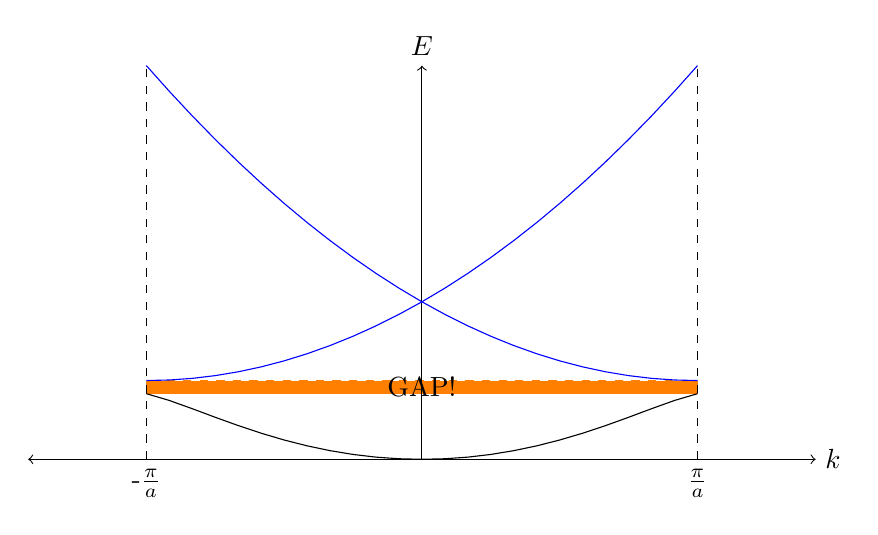
\begin{tikzpicture}[scale=0.5]
        \filldraw[orange, dashed] (-7, {5/3}) rectangle(7, 2);
        \draw[<->] (-10,0) -- (10,0);
        \node[right] at (10,0) {$k$};
        \draw[->] (0,0) -- (0,10);
        \node[above] at (0,10) {$E$};
        \draw[dashed] (-7,0) -- (-7,10);
        \node[below] at (-7,0) {-$\frac{\pi}{a}$};
        \draw[dashed] (7,0) -- (7,10);
        \node[below] at (7,0) {$\frac{\pi}{a}$};
        \draw[domain=-7:7] plot(\x, {\x * \x / 49 * 2 - exp(abs(\x))/(3 * exp(7))});
        \draw[blue, domain=-7:7] plot(\x, {(7 - \x) ^2 / 49 * 2 + 2});
        \draw[blue, domain=-7:7] plot(\x, {(- 7 - \x) ^2 / 49 * 2 + 2});
        \node at (0,11/6) {GAP!};
    \end{tikzpicture}
    \caption{Notice the orange gap with the introduction of a small $V_1$}
    \label{17.9.split}
\end{figure}

Moreover, if we examine the eigenvectors of the matrix we find $\left( 1\;\pm 1 \right)^T$, which look just like standing waves, so the eigenfunctions near this gap look like standing waves.

If we have higher Fourier components of our periodic potential, then we can again apply degenerate perturbation theory to find $2V_2$ gap split; note this occurs at the $k=0$ intersection, because the two $k$ values that interfere are $k = \pm \frac{2\pi}{a}$. More generally, the band structure will be split according to the harmonics of the potential.

\chapter{01/10/14 --- Bloch recap, Deteriming crystal structure}

\section{Recap of everything so far}

Recall that with two atoms with ground state energies $\epsilon_0$ bonding we obtain a bonding and antibonding orbital of $\varepsilon \pm t$ energies respectively. Bloch bands are just the generalization of this, where the energy bands run from $\varepsilon_0 - 2t$ to $\varepsilon_0 + 2t$, a total span of $4t$. The Bloch wavefunction then looks like a periodic function modulated by an overall plane wave $\pi/k$ wavelength. 

The full potential that the electron is subject to in the lattice is given by $V_c(\vec{r}) = -\sum\limits_{}^{}\frac{Ze}{\abs{\vec{r} - \vec{R}}}$. Instead of working with such a difficult potential, we often will work with an effective potential $V_{eff}(\vec{r}) = V_c(\vec{r}) + \Delta V(\vec{r})$ with $\Delta V$ some mean field approximation of everything else.

One such approximation is the \emph{Hartree potential}, which is given $V_H(\vec{r}) = \int\limits_{}^{}dr'\;\frac{e}{\abs{\vec{r} - \pvec{r}}}\rho(\pvec{r})$. A further approximation can be given by some exchange potential $V_{XC}(\vec{r})$, and the full theory of these approximations makes up DFT, density functional theory.

Let's roughly cover what we will talk about in the PC. We expand the Bloch function 
\begin{align}
    \psi_{\vec{k}}(\vec{r}) = u_{\vec{k}}(\vec{r})e^{i\vec{k} \cdot \vec{r}} = \sum\limits_{\vec{G}}^{}u_{\vec{k};\vec{G}}e^{i\left( \vec{G} + \vec{k} \right)\cdot \vec{r}}
\end{align}
for $\vec{G}$ in the reciprocal lattice. This is very important expansion, because the true momentum of the electron can have any values $\vec{k} + \vec{G}$. We refer to $\vec{k}$ as the \emph{quasi-momentum} of the electron; we often refer to this as the momentum of the electron, but it is important to remember it can take on any of the momentum values given by $\vec{k} + \vec{G}$ for $\vec{G}$ in the reciprocal lattice as happens in the Fourier decomposition.

We then have an independent eigenvalue problem at each $k$, which is given by 
\begin{align}
    \sum\limits_{G'}^{}M_{G,G'}^{(k)}u_{k;G'} = \epsilon_k u_{k;G}
\end{align}
with $M$ representing the Fourier modes of the Hamiltonian (recall that for a cosine potential we had a ``tri-diagonal'' matrix), or more specifically
\begin{align}
    M_{G,G'}^{(k)} = \frac{\hbar^2}{2m}\left( k + G \right)^2 \delta_{GG'} + V_{G-G'}
\end{align}

This is not very suitable for our Coulomb problem, because trying to expand such a potential in Fourier modes will require very many terms, and so $M$ will be a very complicated matrix. Specifically, for orbitals closer to the nucleus the potential becomes poorly modeled when the Fourier series is truncated. In light of this problem we have spent many decades trying to get around this, such as doing the Fourier expansion for only the valence electrons (which are further from the nucleus in general) while doing something else for the inner electrons. We will not delve deeply into this in this course, thankfully.

Recall also that in the weak potential approximation, we ``fold the parabola'' in wavenumber space (the parabola being $\frac{\hbar^2 k^2}{2m}$) and we obtain gaps based on the Fourier components (this was the last PC). How does this relate to the tight-binding picture? We note for a stronger potential this first gap becomes larger as well, and gradually we become better described by bonding/antibonding orbitals rather than this weak potential splitting (I think it means you can view the bottom two bands of the energy states as the bonding and antibonding orbitals respectively).

This terminates the overview of what we should know up to this point.

\section{Determining crystal structure of a material}

We want to be able to probe the exact coordinates of atoms within a crystal. We know that the separation of these atoms is on the order of \AA, and we know we must probe with \emph{something}, something with wavelength on the order of \AA\@ as well. Xrays fit this perfectly, as well as neutrons. Photons will interact with the electrons while neutrons interact strongly with nuclei because spin/magnetic moment. Note that neutrons probe magnetic properties of the materials too which is inaccessible to photon diffraction!

To obtain high-resolution x-ray diffractions we use synchrotrons, which accelerate electrons really fast. This gives off coherent radiation. To generate neutrons for neutron diffraction we must induce nuclear reactions; there are a few of these around the world.

Let's cover the basic theory for xray diffraction. We have an incident electron at $\vec{k}_0$ and a refracted electron $\vec{k}_1$. Suppose we are colliding elastically, then $\abs{\vec{k}_0} = \abs{\vec{k}_1} = \frac{2\pi}{\lambda}$. We will not consider the amplitude ratio of the incoming and outgoing waves, because this depends specifically on the scattering process, but let's call this $\alpha_{k_0, k_1}$.

The outgoing photon then looks like 
\begin{align}
    \psi_{0,out} &= A_0 \alpha_{k_1, k_2} e^{i\left( \vec{k}_1 \cdot \vec{r} - \omega t \right)}
\end{align}

We then want the phase change in scattering off an atom $\vec{R}$ away, with $\vec{R}$ the Bravais lattice translation vector thing. We want the phase difference that results in this different path, depicted in \ref{01.10.1}
\begin{figure}[!h]
    \centering
    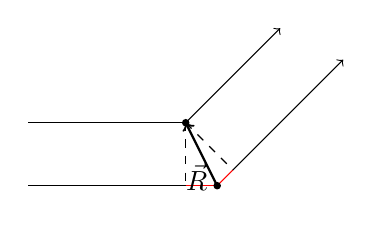
\begin{tikzpicture}[scale=0.2]
        \draw (-10,0) -- (0,0);
        \draw[red] (0,0) -- (2,0);
        \draw[red] (2,0) -- (3,1);
        \draw[->] (3,1) -- (10,8);
        \draw (-10,4) -- (0,4);
        \draw[->] (0,4) -- (6,10);
        \draw[dashed] (0,4) -- (0,0);
        \draw[dashed] (0,4) -- (3,1);
        \filldraw (2,0) circle(0.2);
        \filldraw (0,4) circle(0.2);
        \draw[thick, <-] (0,4) -- (2,0);
        \node[below] at (0.7,2) {$\vec{R}$};
    \end{tikzpicture}
    \caption{Path difference in scattering off a site $\vec{R}$ away, highlighted in red.}
    \label{01.10.1}
\end{figure}

It turns out with a bit of geometry that this path difference is just $\left( \vec{k}_1 - \vec{k}_0 \right) \cdot \vec{R} = \frac{2\pi}{\lambda} d$. Let's define $\vec{K} = \vec{k}_1 - \vec{k}_0$, then we have the outgoing photon at the other site
\begin{align}
    \psi_{1,out} &= A_0 \alpha_{k_1, k_2} e^{i\left( \vec{k}_1 \cdot \vec{r} - \omega t \right)} e^{-i\vec{K} \cdot \vec{r}}
\end{align}

Then if we want the total amplitude we must take a sum of all these amplitudes $A_0 \alpha_{k_0, k_1}\left[ \sum\limits_{\vec{R}}^{}e^{-i\vec{K} \cdot \vec{R}} \right]$. This in general adds destructively, because the phase is arbitrary, but will add constructively when $\vec{K} \cdot \vec{R} = 2\pi$, or in other words when $\vec{K} \in \vec{G}$ in the reciprocal lattice! These points of constructive interference then show up as dark spots on the diffraction pattern, called \emph{Bragg spots}.

This is a very hand-wavy argument; it produces extremely dark and sharp Bragg spots. Instead, we can do this for a finite lattice sum instead, which we will do in the PC, and obtain the widths of the Bragg spots etc.

We can see this in a much more intuitive way, the ``English way'' rather than the French (YES!!)\footnote{The French formulation, the more accepted one nowadays, is called the Von La\"ue formulation}. We can decompose a lattice into sheets (``reticular plane''), and if we treat the sheets as mirrors we have a reflection about the normal to the planes. Then if we simply draw this picture out as in \ref{01.10.2} we again recover this path difference, which in this case is the condition $2d\sin\theta = n\lambda$.
\begin{figure}[!h]
    \centering
    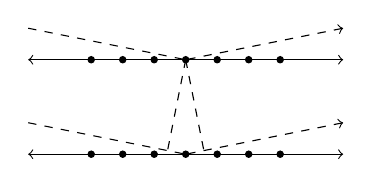
\begin{tikzpicture}[scale=0.2]
        \draw[<->] (-10,3) -- (10,3);
        \draw[<->] (-10,-3) -- (10,-3);
        \draw[dashed] (-10,5) -- (0,3); 
        \draw[dashed, <- ] (10,5) -- (0,3); 
        \draw[dashed] (-10,-1) -- (0,-3); 
        \draw[dashed, <- ] (10,-1) -- (0,-3); 
        \draw[dashed] (0,3) -- (-1.16,-2.8);
        \draw[dashed] (0,3) -- (1.16,-2.8);
        \filldraw (0,3) circle(0.2);
        \filldraw (2,3) circle(0.2);
        \filldraw (4,3) circle(0.2);
        \filldraw (6,3) circle(0.2);
        \filldraw (-2,3) circle(0.2);
        \filldraw (-6,3) circle(0.2);
        \filldraw (-4,3) circle(0.2);
        \filldraw (0,-3) circle(0.2);
        \filldraw (2,-3) circle(0.2);
        \filldraw (4,-3) circle(0.2);
        \filldraw (6,-3) circle(0.2);
        \filldraw (-2,-3) circle(0.2);
        \filldraw (-6,-3) circle(0.2);
        \filldraw (-4,-3) circle(0.2);
    \end{tikzpicture}
    \caption{Bragg's version of these Bragg spots}
    \label{01.10.2}
\end{figure}

That this is equivalent to the reciprocal lattice formulation is a slightly more difficult proof; we can find this online.

We can also generalize this to several atoms per unit cell. It turns out for xray diffraction the spots are just the Fourier transform of the electron density!

\chapter{01/10/14 --- PC 3 --- Direct/Reciprocal Lattice}

\section{Vocabulary}

\begin{itemize}
    \item Bravais Lattice --- $\vec{R} = n_i\vec{a}_i$ such that $\vec{a}_i$ are linearly independent.
    \item Basis/motif --- The contents of each unit cell. We prefer motif, but in many books it is called basis.
    \item Unit Cell --- Volume of space such that when translated through vectors of Bravais lattice fills space without overlapping itself
    \item Wigner-Seitz cell --- Unit cell comprising points that are closer to a single lattice point than any other lattice point. Typically, we accomplish this by bisecting the sides of the unit cell and joining the resulting figure (e.g. $\left[ \pm \frac{1}{2}  \right]^n$ is the set of points closest to the origin if Cartesian lattice points are Bravais lattice). Volume is $\frac{1}{n}$ with $n$ density of Bravais lattice points.
    \item Reciprocal lattice --- $\vec{G}: \left\{ \vec{g} \in \vec{G}, \vec{r} \in \vec{R}, e^{i \vec{g} \cdot \vec{r}} = 1 \right\}$.
    \item First Brillioun Zone --- Wigner-Seitz unit cell of the reciprocal lattice centered around $\vec{0}$, or $\vec{k} \in \left[ -\frac{\pi}{a}, \frac{\pi}{a} \right]^n$.

        Note that size of unit cell in reciprocal lattice is $\tilde{V} = \frac{\left( 2\pi \right)^n}{V}$.
\end{itemize}

\section{Reciprocal lattice and xray diffraction}

\begin{enumerate}[1.]
    \item \emph{What are the reciprocal lattices of simple cubic, fcc, and bcc?}

        We know that if the Bravais Lattice can be written $n_i\vec{a}_i$ and the reciprocal lattice $n_i\vec{b}_i$, then the explicit forms for the $\vec{b}_i$ in terms of the $\vec{a}_i$ is
        \begin{align}
            \vec{b}_1 &= \frac{2\pi\left( \vec{a}_2 \times \vec{a}_3 \right)}{\vec{a}_1 \cdot \left( \vec{a}_2 \times \vec{a}_3 \right)}&
            \vec{b}_2 &= \frac{2\pi\left( \vec{a}_3 \times \vec{a}_1 \right)}{\vec{a}_1 \cdot \left( \vec{a}_2 \times \vec{a}_3 \right)}&
            \vec{b}_3 &= \frac{2\pi\left( \vec{a}_1 \times \vec{a}_2 \right)}{\vec{a}_1 \cdot \left( \vec{a}_2 \times \vec{a}_3 \right)}
        \end{align}
        
        One may verify that $\vec{a}_i \cdot \vec{b}_j = 2\pi \delta_{ij}$. 

        \begin{enumerate}[a)]
            \item Simple Cubic: $\vec{a}_1 = a\hat{x}, \vec{a}_2 = a\hat{y}, \vec{a}_3 = a\hat{z}$ which produces
                \begin{align}
                    \vec{b}_1 &= \frac{2\pi \hat{x}}{a}&
                    \vec{b}_2 &= \frac{2\pi \hat{y}}{a}&
                    \vec{b}_3 &= \frac{2\pi \hat{z}}{a}
                \end{align}
            \item Face-centered cubic (fcc): We have $\vec{a}_1 = \frac{a}{2}\left( \hat{y} + \hat{z} \right), \vec{a}_2 = \frac{a}{2}\left( \hat{x} + \hat{z} \right), \vec{a}_3 = \frac{a}{2}\left( \hat{x} + \hat{y} \right)$, so plug and choo choo!
                \begin{align}
                    \vec{b}_1 &= \frac{2\pi}{a}\left( \hat{y} + \hat{z}  - \hat{x}\right)&
                    \vec{b}_2 &= \frac{2\pi}{a}\left( \hat{x} + \hat{z}  - \hat{y}\right)&
                    \vec{b}_3 &= \frac{2\pi}{a}\left( \hat{x} + \hat{y}  - \hat{z}\right)
                \end{align}
            \item Body-centered cubic: We have many choices here, but we will choose $\vec{a}_1 = \frac{a}{2}\left( \hat{y} + \hat{z} - \hat{x} \right), \vec{a}_2 = \frac{a}{2}\left( \hat{z} + \hat{x} - \hat{y} \right), \vec{a}_3 = a\left( \hat{x} + \hat{y} - \hat{z} \right)$. 
                
                Note however that these are exactly the Bravais lattice vectors for fcc! Then an fcc with cube side length $a$ has reciprocal lattice with unit cell side length $\frac{4\pi}{a}$. 
        \end{enumerate}

    \item \emph{Each family of retular planes is labeled by three integers $(h,k,l)$ called Miller indicies such that each plane in the family cuts the axes $\vec{a}, \vec{b}, \vec{c}$ at $\frac{n}{h}, \frac{n}{k}, \frac{n}{l}$. Show that the planes are perpendicular to the reciprocal lattice vector $\vec{K}_{hkl} = h\vec{a}^{\,*} + k\vec{b}^{\,*} + l\vec{c}^{\,*}$}

        Let's first examine a vector $\vec{x}$ in the $n=0$ plane with some Miller index. Let $\vec{s}$ be the normal to this $n=0$ plane, then $\vec{x} \cdot \vec{s} = 0$. But then if we take a vector $\vec{x}$ in a $n\neq0$ plane with the same Miller index, we obtain that $\vec{x} \cdot \pvec{s}= C_m$ with $C_m$ the distance between the planes (let them be separated by $m$ planes). 

        Then we know that $\vec{a} \cdot \hat{s} = A(n)\frac{h}{n}$, because $\frac{n}{h}\vec{a}$ is on the $n$-th plane. Finally, if we expand $\hat{s}$ in the reciprocal lattice $\hat{s} = s_a^*\vec{a}^{\,*} + s_b^*\vec{b}^{\,*} + s_c^*\vec{c}^{\,*}$. By then dotting $\vec{a}, \vec{b}, \vec{c}$ against $\hat{s}$ we find the components of $\hat{s}$ to be
        \begin{align}
            s_a^* &= \frac{A(n)h}{2\pi n}&
            s_b^* &= \frac{A(n)k}{2\pi n}&
            s_c^* &= \frac{A(n)l}{2\pi n}
        \end{align}
        which then solving gives us that $\left\{ h,k,l \right\} = \frac{2\pi n}{A(n)}\left\{ s_a^*, s_b^*, s_c^* \right\}$ and so we find $\vec{K}_{hkl} \parallel \hat{s}$. 
    \item \emph{Show that the distance $d_{hkl}$ between two neighboring planes is inversely proportional to $\vec{K}_{hkl}$}

        This is given in our above expression, where we find $\abs{\vec{K}_{hkl}} \propto A^{-1}(n)$. More specifically then, $d_{hkl} = \frac{2\pi}{\abs{\vec{K}_{hkl}}} = \frac{2\pi}{\abs{\vec{k}_i}\sin\theta_{hkl}}$ with $\theta_{hkl}$ the angle of incidence of incoming beam (I'm mixing and matching a bit).
    \item \emph{Show the Bragg reflection conditions $\abs{\vec{k}_i} = \abs{\vec{k}_i + \vec{K}_{hkl}}$ is the same thing $2d_{hkl} \sin \theta_{hkl} = n\lambda$.}

        We already have $\abs{\vec{k}_i} = \frac{2\pi}{\lambda}$, and then in conjunction with our earlier result we obtain $\lambda = 2d_{hkl}\sin\theta_{hkl}$. Then of course $d_{hkl}$ only includes the Bravais lattice separation, and since we have larger separations still in reciprocal space we must include these higher multiples. These higher mulitples are $n$ times $d_{hkl}$ (the shortest Bravais lattice vector) and so we obtain our final expression
        \begin{align}
            n\lambda = 2d_{hkl}\sin\theta_{hkl}
        \end{align}
\end{enumerate}

\chapter{08/10/14 --- Makeup:Multiple electrons}

We have been discussing the single electron wavefunction case for all the systems thusfar. With $N$ electrons, we need more information. Since electrons are fermions, we need an antisymmetric wavefunction, so we begin with a Slater determinant
\begin{align}
    \Psi\left( \left\{ \vec{r}_i \right\} \right) = \det\left[ \psi_{\alpha_i}\left( \vec{r}_j \right) \right]
\end{align}
with $\alpha_n = \vec{k_n},\nu_n, \sigma_n$ orbital characteristics ($\sigma$ is spin).

Note that despite the fact the electrons are treated as independent, we still know that they obey Pauli Exclusion Principle. The way that electrons are promoted from some energy $\epsilon_i \to \epsilon_f$ costs $\epsilon_f - \epsilon_i$ and is called a \emph{particle-hole excitation} which conserves number of particles. Given this, let's try to extrapolate to the energy spectrum of a solid.

Let us have $N_{at}$ hydrogen atoms and $N$ electrons. Then $N < N_{at}$ electrons will partially fill the lower band, because recall that $\frac{N_{at}}{2}$ energy levels can accomodate $N_{at}$ electrons because of spin. If we have even $\frac{N}{N_{at}}$ then we have an insulator, beacuse every energy band is filled (each energy band has $2N_{at}$ holes for electrons).

\section{Fermi Level}

We define $\epsilon_F$ the highest occupied energy state in the ground state of the system the \emph{Fermi Energy}. The ground state is called the \emph{Fermi Sea}. We call the surface of electrons at $\epsilon_F$ in $\vec{k}$ space the \emph{Fermi surface}; electrons on this surface will react to excitations. In an insulator, we note that the Fermi Energy must fall in the middle of the gap between energy levels, and so the Fermi surface is open (no electrons lie in the gap). 

\section{Density of States}

We want to count the number of states as the band structure becomes infinitely dense. This is given
\begin{align}
    D_{\nu\sigma}(\epsilon) &= \int\limits_{BZ}^{}\frac{d^dk}{V_{BZ}}\delta\left( \epsilon - \epsilon_{\vec{k}\nu,\sigma} \right)
\end{align}
with $\sigma = \uparrow, \downarrow$ the spin.

This is nice because $\int\limits_{-\infty}^{\infty}d\epsilon\;D_{\nu\sigma}(\epsilon) = 1$.

Note that if we plot $D(\epsilon)$ as a function of $\epsilon$ we have many states within a given $\delta \epsilon$ level if the curve is relatively flat there.

I can't take any more notes because I don't understand Cedric's notes :(.

\chapter{08/10/14 + 15/10/14 --- PC 4 + 5 --- Graphene}

Allotropes of carbon exist in all dimensions (macroscopically speaking):
\begin{itemize}
    \item 0D --- Fullerene
    \item 1D --- Nanotube
    \item 2D --- Graphene
    \item 3D --- Graphite, diamond
\end{itemize}

In graphene, the orbitals are $sp_2$ hybridized, so $120^\circ$ planar bonds. The remaining $p_z$ orbital bonds as a $\pi$ bond.

\begin{enumerate}[1.]
    \item \emph{Characterize the crystal by its Bravais lattice and its motif/basis.}

        We note we have a honeycomb structure, so we simply choose a scale and find $\vec{a}_1 = \hat{x}, \hat{a}_2 = \frac{\hat{x}}{2} + \frac{\hat{y}\sqrt{3}}{2}$. The motif is simply the two-atom link $\frac{\hat{x}}{2} + \frac{\hat{y}\sqrt{3}}{4}$. 

    \item \emph{Represent graphically the reciprocal lattice.}

        First let's recall the formula $\vec{b}_1 = \frac{2\pi\left( \vec{a}_2 \times \vec{a}_3 \right)}{\vec{a}_1 \cdot \left( \vec{a}_2 \times \vec{a}_3 \right)}$ and its cyclic permutations. We will just take $\vec{a}_3 = \hat{z}$, as the magnitude cancels, and so we find that
        \begin{align}
            \vec{b}_1 &= \frac{4\pi \left( -\frac{\hat{x}\sqrt{3}}{2} + \frac{\hat{y}}{2} \right)}{\abs{\vec{a}_1}}\\
            &= 4\pi \left( -\frac{\hat{x}\sqrt{3}}{2} + \frac{\hat{y}}{2} \right)\\
            \vec{b}_2 &= 4\pi\hat{y}
        \end{align}

        So we can draw this little mofo
        \begin{figure}[!h]
            \centering
            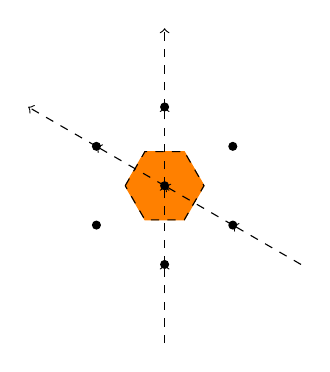
\begin{tikzpicture}
                \filldraw[orange] (-1/2,0) -- (-1/4,{sqrt(3)/4}) -- (1/4,{sqrt(3)/4}) -- (1/2,0) -- (1/4,{-sqrt(3)/4}) -- (-1/4,{-sqrt(3)/4}) -- (-1/2,0);
                \draw[dashed] (-1/2,0) -- (-1/4,{sqrt(3)/4}) -- (1/4,{sqrt(3)/4}) -- (1/2,0) -- (1/4,{-sqrt(3)/4}) -- (-1/4,{-sqrt(3)/4}) -- (-1/2,0);
                \draw[->, dashed] (0,0) -- (0,1);
                \draw[->, dashed] (0,1) -- (0,2);
                \draw[->, dashed] (0,-1) -- (0,0);
                \draw[->, dashed] (0,-2) -- (0,-1);
                \draw[->, dashed] (0,0) -- ({-sqrt(3)/2},1/2);
                \draw[->, dashed] ({-sqrt(3)/2},1/2) -- ({2 * (-sqrt(3)/2)},2/2);
                \draw[->, dashed] ({sqrt(3)/2},-1/2) -- (0,0);
                \draw[->, dashed] ({sqrt(3)},-1) -- ({sqrt(3)/2},-1/2);
                \filldraw ({sqrt(3)/2},1/2) circle(0.05);
                \filldraw ({-sqrt(3)/2},-1/2) circle(0.05);
                \filldraw ({-sqrt(3)/2},1/2) circle(0.05);
                \filldraw ({sqrt(3)/2},-1/2) circle(0.05);
                \filldraw (0,1) circle(0.05);
                \filldraw (0,-1) circle(0.05);
                \filldraw (0,0) circle(0.05);
            \end{tikzpicture}
            \caption{Reciprocal lattice; dots mark the lattice points and vectors mark the lattice vectors. First Brillioun Zone is shaded, Wigner-Seitz unit cell in reciprocal lattice.}
            \label{08.10.lattice}
        \end{figure}

        Note that the reciprocal lattice cares only about the Bravais lattice, not the motif/basis. Recall also that diffraction highlights the reciprocal lattice points; the way we find out that there are multiple atoms in the unit cell/motif we will see a variation in the intensity distribution at these extrema of the diffraction experiement (otherwise, all points are uniform). 

    \item \emph{Compute the structure factor $S(h,k)$.}

        The structure factor is defined as (slightly different convention from the book; We call $S$ what the book calls $A(\vec{G}) = S(\vec{G}) \cdot \sum\limits_{n}^{}e^{i\vec{G} \cdot \vec{R}_l}$)
        \begin{align}
            S(\vec{G}) &= \sum\limits_{l}^{}f_l(\vec{G}) e^{-i\vec{G}\cdot \vec{R}_l}\\
            &= \sum\limits_{l}^{}\int\limits_{}^{}du\;\rho(u)e^{-i\vec{u} \cdot \vec{G}}e^{-i\vec{G} \cdot \vec{R}_l}
        \end{align}
        where $f_l(\vec{G})$ is some function giving phase-included density within the unit cell/motif of some sort, as above.

        We know that $\vec{G} \cdot \vec{R}_l = 2\pi n$ because Bravais lattice (and since the sum runs over Bravais Lattice sites the sum evaluates to $\frac{N}{2}$ with $N$ number of atoms), and the integral only spans two sites of atoms, so our structure factor becomes (with $\vec{d}$ the vector separating the motif)
        \begin{align}
            S(\vec{G}) &= \frac{N}{2}\left( 1 + e^{-i \vec{G} \cdot \vec{d}} \right)\\
            \vec{G} \cdot \vec{d} &= \left( h\vec{b}_1 + k\vec{b}_2 \right) \frac{\left( \vec{a}_1 + \vec{a}_2 \right)}{3} = \frac{2\pi}{3}\left( h + k \right)\\
            &= \frac{N}{2}\left( 1 + e^{-i\frac{2\pi}{3}\left( h + k \right)} \right)\\
            I = \abs{S}^2 &= \frac{N^2}{4}\left( 2 + 2\cos \frac{2\pi(h+k)}{3} \right)
        \end{align}

        Since $h,k\in\mathbb{Z}, \cos \frac{2\pi \mathbb{Z}}{3} = 1,-\frac{1}{2}$, and so $I = N^2, \frac{N^2}{4}$, and indeed we find that at sites $\vec{G}$ for which $3 | (h+k)$ we find these sites will be stronger signal.

    \item \emph{Now assume tight binding, so diagonal elements are $\epsilon$ and neighboring sites $-t$ and rest $0$. Project the SE onto the space spanned by the eigenstates at the motif sites.}

        Let's write down the SE, ignoring normalization and implicitly summing over repeated index $j$ (let $\ket{A_j}, \ket{B_j}$ represent the eigenstates for motif sites $A,B$ at Bravais Lattice site $j$)\footnote{Our assumed waveform comes from Bloch's theorem.}
        \begin{align}
            H(\lambda_a \ket{A_j} + \lambda_B \ket{B_j}) e^{i\vec{k} \cdot \vec{R}_j} &= E(\lambda_a \ket{A_j} + \lambda_B \ket{B_j}) e^{i\vec{k} \cdot \vec{R}_j}        
        \end{align}

        We can dot both sides alternatively with an $\bra{A_k}, \bra{B_k}$ and we find
        \begin{align}
            \lambda_a \epsilon - \lambda_bt\left( 1 + e^{-i\vec{k} \cdot \vec{a}_1} + e^{-i\vec{k} \cdot \vec{a}_2} \right) &= E\lambda_a\\
            \lambda_b \epsilon - \lambda_at\left( 1 + e^{i\vec{k} \cdot \vec{a}_1} + e^{i\vec{k} \cdot \vec{a}_2} \right) &= E\lambda_b
        \end{align}

        We see this expression by examining the three neighboring $\bra{B_k}$ for a $\ket{A_j}$, which belong to Bravais Lattice sites either $1, -\vec{a}_1, -\vec{a}_2$ away.

    \item \emph{Derive the dispersion relation $E(\vec{k})$.}

        Bash bash
        \begin{align}
            \frac{\lambda_at\left( 1 + e^{i\vec{k} \cdot \vec{a}_1} + e^{i\vec{k} \cdot \vec{a}_2} \right)}{\epsilon - E} &= \lambda_b\\
            \lambda_a \epsilon - \lambda_a\frac{t^2\left( 1 + e^{-i\vec{k} \cdot \vec{a}_1} + e^{-i\vec{k} \cdot \vec{a}_2} \right)\left( 1 + e^{i\vec{k} \cdot \vec{a}_1} + e^{i\vec{k} \cdot \vec{a}_2} \right)}{\epsilon - E} &= E\lambda_a\\
            \epsilon(\epsilon - E) -  t^2\left( 3 + e^{i\vec{k} \cdot \vec{a}_1} + e^{i\vec{k} \cdot \vec{a}_2} - e^{i\vec{k} \cdot \vec{a}_1} - e^{i\vec{k} \cdot \vec{a}_2} + e^{i\vec{k} \cdot \left( \vec{a}_2 - \vec{a}_1 \right)} + e^{-i\vec{k} \cdot \left( \vec{a}_2 - \vec{a}_1 \right)}\right) &= E(\epsilon - E)\\
            t^2\left( 3 + 2\left( \cos \vec{k} \cdot \vec{a}_1  + \cos \vec{k} \cdot \vec{a}_2 + \cos \vec{k} \cdot \left( \vec{a}_1 - \vec{a}_2 \right)\right)\right) &= E^2 - 2E\epsilon + \epsilon^2\\
            \pm t\sqrt{3 + 2\Sigma(\vec{k})} &= E - \epsilon
        \end{align}
        with $\Sigma(\vec{k})$ as defined in the handout (and clear above). 

    \item \emph{Define $\vec{k} = \alpha \vec{b}_1 + \beta \vec{b}_2$. Show some stuff, copied inline below.}
        \begin{itemize}
            \item First, we show that $\alpha = \frac{\vec{k} \cdot \vec{a}_1}{2\pi}, \beta = \frac{\vec{k} \cdot \vec{a}_2}{2\pi}$. This is straightforward; by construction $\vec{a}_i \cdot \vec{b}_j = 2\pi\delta_{ij}$ and we are done (just plug in).
            \item Next, we want to show
                \begin{align}
                    \left( \vec{k} \cdot \vec{a}_1 \right)^2 + \left( \vec{k} \cdot \vec{a}_2 \right)^2 - (\vec{k} \cdot \vec{a}_1)(\vec{k} \cdot \vec{a}_2) &= \frac{1}{4}k^2
                \end{align}
                \emph{Note that on the original handout it says $\frac{9a^2}{4}$ instead of $\frac{1}{4}$ but here we have chosen $a=\frac{1}{\sqrt{3}}$ which is different system from in class}

                We simply examine
                \begin{align}
                    k^2 &= \alpha^216\pi^2 + \beta^216\pi^2 - 2\alpha\beta\vec{b}_1 \cdot \vec{b}_2\\
                    \vec{b}_1 \cdot \vec{b}_2 &= (4\pi)^2\cos \frac{\pi}{3} = 8\pi^2\\
                    k^2 &= 4(\vec{k} \cdot \vec{a}_1)^2 + 4(\vec{k} \cdot \vec{a}_1)^2 + 4\left( \vec{k} \cdot \vec{a}_1 \right)\left( \vec{k} \cdot \vec{a}_2 \right)
                \end{align}
        \end{itemize}
    \item \emph{Evaluate $\lim_{k \to 0}\Sigma(\vec{k})$ and $E - \epsilon$.}

        Baaaaaash
        \begin{align}
            \Sigma(\vec{k}) &= \left( \cos \vec{k} \cdot \vec{a}_1  + \cos \vec{k} \cdot \vec{a}_2 + \cos \vec{k} \cdot \left( \vec{a}_1 - \vec{a}_2 \right)\right)\\
            &= 1 - \frac{\left( \vec{k} \cdot \vec{a}_1 \right)^2}{2} + 1 - \frac{\left( \vec{k} \cdot \vec{a}_2 \right)^2}{2} + 1 - \frac{\left( \vec{k} \cdot (\vec{a}_1 - \vec{a}_2) \right)^2}{2} + O(k^4)\\
            &\approx 3 - \frac{\left( \vec{k} \cdot \vec{a}_1 \right)^2 + \left( \vec{k} \cdot \vec{a}_2 \right)^2 + \left[\left( \vec{k} \cdot \vec{a}_1 \right)^2 + \left( \vec{k} \cdot \vec{a}_2 \right)^2 - 2\left( \vec{k} \cdot \vec{a}_1 \right)\left( \vec{k} \cdot \vec{a}_2 \right)\right]}{2}\\
            &= 3 - \frac{1}{4}k^2
        \end{align}

        From this we conclude that $\lim_{k \to 0}E - \epsilon$ is
        \begin{align}
            E - \epsilon &= \pm t\sqrt{3 + 2\Sigma} = \pm t\sqrt{9 - k^2}\\
            &\approx \pm t\left( 3 - \frac{1}{4}k^2 \right)
        \end{align}
        which agrees with the class result $E-\epsilon = -3t + \frac{3}{4}ta^2k^2$ given our choice of $a$. 
    \item \emph{Where does $E - \epsilon$ vanish? (no longer in the small $k$ approximation!)}
        
        Let's go way back, instead of solving cosines (since we aren't in the small $k$ approximation cosines suck) and use the full exponential expression
        \begin{align}
            E - \epsilon &= \pm t\sqrt{\left( 1 + e^{i\vec{k}\cdot\vec{a}_1} + e^{i\vec{k}\cdot\vec{a}_2} \right)\left( 1 + e^{-i\vec{k}\cdot\vec{a}_1} + e^{-i\vec{k}\cdot\vec{a}_2} \right)} = \pm t\abs{1 + e^{i\vec{k}\cdot\vec{a}_1} + e^{i\vec{k}\cdot\vec{a}_2}}
        \end{align}
        which setting equal to $0$ gives us
        \begin{align}
            \cos \vec{k} \cdot \vec{a}_1 + \cos \vec{k} \cdot \vec{a}_2 &= -1\\
            \sin  \vec{k} \cdot \vec{a}_1 + \sin \vec{k} \cdot \vec{a}_2 &= 0
        \end{align}

        Call $\vec{k} \cdot \vec{a}_1 = x, \vec{k} \cdot \vec{a}_2 = y$. We then require $\sin x = -\sin y, \cos x \neq \cos y$ which gives us that $x=-y$. Then plugging into the first equation gives us that $x = y = \pm\frac{2\pi}{3} + 2\pi n$, and so we find that
        \begin{align}
            \alpha &= \pm \frac{1}{3} + n & \beta &= \mp \frac{1}{3} + n
        \end{align}

        This produces $6$ points on the edge of the Brillouin Zone, each one one vertex of the hexagon.

    \item \emph{Show that in the neighborhood of these points the energy goes linearly like $E = \pm \frac{3}{2}ta\abs{\vec{k} - \vec{k}_p}$.}

        Hahahahahaha, we get to take this for granted! (This shows up on the energy levels because where the gap vanishes the energy levels around go linearly).
    \item \emph{Calculate the density of states around $E = 0$.}

        Recall the definition of the density of states $\rho(\epsilon) = \frac{1}{\Omega_{BZ}}\sum\limits_{k \in BZ}^{} \delta(\epsilon - \epsilon_k)$ with $\Omega_{BZ}$ the volume of the BZ. Long story short the density of states measures the degeneracy of states within an interval $dE$ so we have a measure when integrating $dE$, such as $\expvalue{A} = \int dN\; A(N) = \int dE\; f(E) \rho(E) A(E)$ with $f(E)$ measuring the occupancy and $\rho(E)$ measuring the number of states available.

        Let's denote our result from the previous section $E = \pm v_F \abs{K}$ with $v_F$ the \emph{Fermi velocity}. We then just plug into our integral
        \begin{align}
            \rho(\epsilon) &= \frac{1}{\Omega}\int d\vec{k}\; \delta(\epsilon - \epsilon_k)
        \end{align}

        We go to polar coordinates and we resolve a small subtlety: since there are $6$ such cones, and each one lies at the boundary of $3$ BZs, we must insert a factor of $2$ because each BZ has two total cones. This gives us that
        \begin{align}
            \rho(\epsilon) &= \frac{1}{\Omega}\int dk\; k \cdot 2\pi \delta(\epsilon - v_Fk)\\
            &= \frac{4\pi}{\Omega}\int dk\; k\delta\left( \epsilon - N_F k \right)\\
            &= \frac{4\pi}{\Omega v_F^2}\epsilon = \frac{2\sqrt{3}}{3t^2\pi}\epsilon
        \end{align}

        We performed this calculation for positive $\epsilon$ (this is hidden in our writitng $\delta(\epsilon - \epsilon_k)$ as $\delta$ functions are symmetric up to a sign in the argument); if we perform for negative $\epsilon$ we find that a negative sign falls out and so in the end $\rho(\epsilon) \sim \abs{\epsilon}$. This is an unusual density of states because $\rho(\epsilon)$ rarely ever vanishes at $\epsilon = 0$. 
        
    \item \emph{How does the specific heat behave at low temperature, in the half-filled case?}

        Recall that $c_V = \pd{U}{T}, U = \int d\epsilon\; \rho(\epsilon) f(\epsilon)\epsilon$. Moreover, at low temperatures $f(\epsilon) \approx \theta(-\epsilon)$ the Heaviside step. So we have
        \begin{align}
            U(T) - U(T=0) &= \int\limits_{-\infty}^{\infty}d\epsilon\;\rho(\epsilon) \left( f(\epsilon) - \theta(-\epsilon) \right)\epsilon\\
            &\sim 2\int\limits_0^{\infty}d\epsilon\;\epsilon\abs{\epsilon} \frac{1}{1 + e^{\beta\epsilon}}
        \end{align}
        where we take advantage of the evenness of the function to drop the step function. We introduce $x = \beta\epsilon$ ($\beta$ is whatever is inside the Fermi-Dirac that we're too lazy to work with)
        \begin{align}
            U(T) - U(T=) &\sim \frac{1}{\beta^2} \int\limits_{0}^{\infty}\frac{x^2}{1 + e^x}\;dx\\
            &\sim \beta^3 \sim T^3
        \end{align}
        and so we find that $C_V \sim T^2$ which is very unusual, and arises due to the $\rho(\epsilon) \sim \abs{\epsilon}$. 
\end{enumerate}

One last note why graphene is cool. Near $E=0$ we recall that $E \sim \abs{k}$. In a free particle, we have $E \sim k^2$, and through this we realize that $E\sim \abs{k}$ is closer to massless particles which obey $E=\hbar ck$. We then see that the electrons in graphene obey like light particles, Dirac physics, with speed of light $\sim v_F$. The cones in reciprocal space are called Dirac cones. 
\chapter{15/10/14 --- More band structures, semiconductors}

\section{Band structures of various types of structures}

We begin by examining a simple metal, sodium. Recall that sodium has $1$ valence electron. In terms of simple qualitative terms, we find that the 1s orbitals are almost entirely localized in the metal, while higher orbitals are much easier split and overlap more heavily in their orbital wavefunctions. This manifests itself in that the valence electron, in the 3s orbital, is almost entirely delocalized between two neighboring atoms. 

Sodium manifests itself as a bcc, and so in reciprocal space it looks like an fcc. The Fermi surface is completely inside the first Brillouin Zone, which is a helpful situation because the borders of the Brillouin Zone are prone to Bragg electron reflection and incur level splitting. If we plot the energy levels with respect to $k$ we find that the 1s, 2s orbitals split very nicely, but the 3s, 3p energy levels overlap heavily at the boundary of the Brillouin Zone. We remedy this in fact by hybridizing the orbitals at the boundaries such that the energy level overlap disappears; these hybridized orbitals are very 3s(3p) in the middle of the Brillouin Zone but take on a much more mixed character at the edges. Often we depict this character by giving the energy bands a thickness corresponding to its 3s quantity, $\abs{\dotp{\psi}{3s}}^2$.

If we examine a more complex metal, such as copper, with $10$ 3d electrons and $1$ 4s electron, we find that the Fermi surface comes close to the boundary of the Brillouin Zone, and consequently the Fermi surface deforms at these boundaries (the way it does so is kinda like one of those suction cups sticking onto the boundary).

We next look at ionic insulators, such as NaCl. By examining plots, we note that the orbital overlap is tiny, and the resulting band structures are very flat because they are localized and atomic in nature.

For covalent insulators, such as diamond, we have very complicated-looking band structures but the bands fall into two large bonding-antibonding chunks separated by a large gap. Evidence of hybridization is evident in that the individual bands all exhibit both s and p characteristics.

\section{Semiconductors}

Semiconductors are characterised by the energy gap in their band structure between bands. We will try to characterize this via the density of states, which will look something like Figure \ref{15.10.DoS}
\begin{figure}[!h]
    \centering
    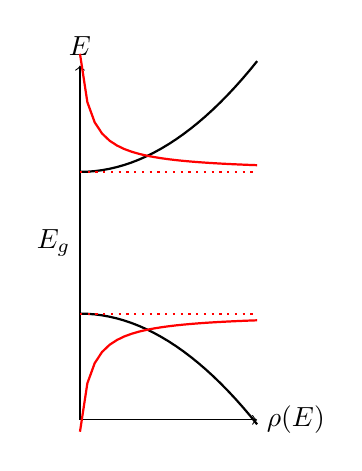
\begin{tikzpicture}[scale=0.45]
        \draw[->] (0,0) -- (5,0);
        \node[right] at (5,0) {$\rho(E)$};
        \draw[->] (0,0) -- (0,10);
        \node[above] at (0,10) {$E$};
        \draw[thick, domain=0:5] plot(\x, \x*\x/8 + 7);
        \draw[thick, domain=0:5] plot(\x, -\x*\x/8 + 3);
        \draw[thick] (0,3) -- (0,7);
        \draw[thick,red, domain=0:5] plot(\x, {1/(\x + 0.3) + 7});
        \draw[thick,red, dotted] (0,3) -- (5,3);
        \draw[thick,red, domain=0:5] plot(\x, {-1/(\x + 0.3) + 3});
        \draw[thick,red, dotted] (0,7) -- (5,7);
        \node[left] at (0,5) {$E_g$};
    \end{tikzpicture}
    \caption{Density of states of a semiconductor. The black is 3D and the red is 1D. The energy gap is the part ine the middle, and the top/bottom bands are the conduction/valence bands respectively.}
    \label{15.10.DoS}
\end{figure}

Note that there are some electrons that can tunnel across this border, into the conduction band, on the order of $e^{-\frac{E_g}{2kT}}$. The difference qualitatively for a semiconductor versus insulator is that $E_g$ is sufficiently small that this exponential isn't strictly nonnegligible at room temperature, somewhere $E_g \lesssim 2\mathrm{eV}$. This tends to result in a measurable resistance rather than infinite.

However, do not compare this with resistance in metals! Recall that in metals $T\uparrow \to \rho \uparrow$ but while in in semiconductors the opposite happens with increasing temperature! This is because semiconductors have a much more pronounced effect in changing number of charge carriers which dominates the decreased mean free path.

\section{Computing number of charge carriers}

Let's try to do some actual calculations. We will begin with some definitions. Call the valence/conduction densities of states $D_v, D_c$ with the number of holes in the valence band $p(T)$ and the number of transferred electrons $n(T)$ and there some chemical potential in the middle $\mu$. 

Recall that $n(T) = \int\limits_{-\infty}^{\infty}D_c(\epsilon) f(\epsilon)\;d\epsilon$ with $f(\epsilon) = \frac{1}{1 + e^{(\epsilon - \mu)/kT}}$ the Fermi-Dirac distribution. Similarly, $p(T) = \int\limits_{-\infty}^{\infty}D_v(\epsilon)\left( 1 - f(\epsilon) \right)\;d\epsilon$. We choose to work in the regime $kT \ll E_g$, and we will assume that $\mu$ isn't too close to either $\epsilon_v, \epsilon_c$ the boundaries of the two bands. Then depending on which regime we are in we have in the large $(\epsilon - \mu)$ limit ($\epsilon - \mu) \sim E_g$)
\begin{align}
    f(\epsilon) &\simeq e^{-(\epsilon - \mu)/kT} & \epsilon > \epsilon_c\\
    1 - f(\epsilon) &\simeq e^{-(\mu- \epsilon )/kT} & \epsilon < \epsilon_c
\end{align}

This finally allows us to write out our integral (we make change of variable $\epsilon' = \epsilon - \epsilon_c$)
\begin{align}
    n(T) &= \int\limits_{-\epsilon_c}^{\infty}D_c(\epsilon)e^{-(\epsilon - \mu)/kT}\;d\epsilon\\
    &= \int\limits_{0}^{\infty}D_c(\epsilon_c + \epsilon')e^{-(\epsilon' + \epsilon_c - \mu)/kT}\;d\epsilon\\
    &= e^{-(\epsilon_c - \mu)/kT} \int\limits_{0}^{\infty}D_c(\epsilon_c + \epsilon)e^{-\epsilon/kT}\;d\epsilon\\
    &= e^{-(\epsilon_c - \mu)/kT}N_c(T)
\end{align}
where we define $N_c(T)$ to be the total number of states in the conduction band. Similarly, we find for $p(T)$
\begin{align}
    p(T) &= N_v(T)e^{-(\mu - \epsilon_v)/kT} & N_v(T) &= \int\limits_{0}^{\infty}D_v(\epsilon_v - \epsilon)e^{-\epsilon/kT}\;d\epsilon
\end{align}

On a side note, one will note that $n(T)p(T) = N_c(T)N_v(T)e^{-E_g/kT}$ doesn't depend on $\mu$! This is called the \emph{mass action law}. In the intrinsic semiconductor case, we also note that $n(T) = p(T)$, because each electron should leave behind a hole. Then we find that $n(T) = p(T) = \sqrt{N_c(T)N_v(T)}e^{-\frac{E_g}{2kT}}$, which doesn't depend on the chemical potential and also agrees with what we said earlier about the order of electrons that can tunnel across the gap!

Near the relative extrema of the energy bands we can approximate the band as a parabola $\pm \frac{\hbar^2 k^2}{2m_{v,c}} + \epsilon_{v,c}$ depending on which band we are in. The resulting density of states shows up as
\begin{align}
    D_c(\epsilon) &= \frac{\sqrt{2}m_c^{3/2}}{\pi^2\hbar^3}\sqrt{\epsilon - \epsilon_c}\theta(\epsilon - \epsilon_c)\\
    D_v(\epsilon) &= \frac{\sqrt{2}m_v^{3/2}}{\pi^2\hbar^3}\sqrt{\epsilon_v - \epsilon}\theta(\epsilon_v - \epsilon)
\end{align}
which produces
\begin{align}
    N_c(T) &= \frac{1}{4}\left( \frac{2m_ckT}{\pi \hbar^2} \right)^{3/2} \sim T^{3/2}\\
    N_v(T) &= \frac{1}{4}\left( \frac{2m_vkT}{\pi \hbar^2} \right)^{3/2}
\end{align}

Finally, we can show using the mass action law the full form
\begin{align}
    n(T) = p(T) = \frac{1}{4}\left( \frac{2kT}{\pi \hbar^2} \right)^{3/2}\left( m_cm_v \right)^{3/4}e^{-\frac{E_g}{2kT}}
\end{align}

For Si at room temperature we find that $n(T) = 10^{16}\mathrm{m^{-3}}$ or $1$ carrier per $10^{13}$ Si atoms. This means we need a really pure Si atom to see the intrinsic behavior, on the order of $10^{-13}$ pure!

We can also plug back through and solve for $\mu$, to verify our assumption that $\mu$ is far from the band edges, and we find
\begin{align}
    \frac{\epsilon_c + \epsilon_v}{2} + \frac{3}{4}kT \ln \frac{m_v}{m_c}
\end{align}
which is going to be small assuming $kT$ is small and $m_v \sim m_c$. 

Doping semiconductors is of course what's really interesting, and long story short concentration of dopant (the right word?) allows control of resistivity over wide wide orders of magnitude $\sim 10^{10}$ for small concentrations of dopant. 

\chapter{22/10/14 --- Makeup: Electronic Transport, conductivity}

\section{Drude Model}

We begin by discussing the Drude model, a fully classical theory. The idea is that electrons move like billiards through a lattice, colliding off ions.

We begin with Ohm's Law, $\vec{j} = \sigma \vec{E}$. We want to derive a formula for $\sigma$ from first principles. Obviously, we can't just put electrons in this $\vec{E}$ field because otherwise current increases linearly in time. Collisions help us resolve this problem; let $\tau$ be the average time in between collisions, then we find that the average carrier velocity $\expvalue{\vec{v}} = -e\frac{\vec{E}}{m}\tau$, as $-e\frac{E}{m}$ is the acceleratn due to the field and it is exerted over time $\tau$. Then, we note that $\vec{j} = -ne\expvalue{\vec{v}}$ and so plugging through the definitions we arriveat
\begin{align}
    \sigma &= \frac{ne^2\tau}{m}
\end{align}

This is the Drude model.  It has very many fundamental flaws
\begin{itemize}
    \item The mean free path in the Drude model must be on the order of a few interatomic distances, but in reality we know that the mean free path in good metals is thousands of times longer.
    \item Obviously, not all electrons participate in transport, only the valence ones! 
    \item Note that $m$ isn't well defined relativistically, since the potential modifies $m$.
\end{itemize}

We can try again by equating electron velocity to gas laws $\frac{1}{2}mv^2 = \frac{3}{2}k_BT, l \propto \sqrt{\frac{kT}{m}\tau}$ and performing the same calculations as above. However,
\begin{itemize}
    \item This is equally wrong, as electrons are subject to Fermi statistics and not ideal gas.
    \item This shows marginal promise in that resistivity increases with temperature in real life.
\end{itemize}

Note that purer metals increase conductivity, which neither of our above models accounts for. The temperature dependence actually comes from the phonons produced by the vibrations in the lattice, 

We can again try to apply classical theory to this heat variation though. Thermal gradient produces a heat current such that $\vec{j}_Q = -\kappa \nabla T$. Classically, we derive that $\kappa = \frac{1}{3}C_evl_e$. The Wiedemann-Franz law then states that $\frac{\kappa}{\sigma} = LT$ with $L = \frac{3}{2}\left( \frac{k_B}{e} \right)$. Remarkably, this is correct up to a factor of $2$. 

The reason that this is wrong is that while $C_e = \frac{3}{2}k_B$ classically (using ideal gas), in QM we find $C_e \sim T$ while the velocity of the electrons goes like the Fermi Velocity, which is independent of temperature. So the temperature dependence pops up in the wrong term, which incredibly gives the correct total result! The factor of $2$ that we are incorrect by arises because instead of $\frac{1}{2}mv^2 = \frac{3}{2}k_BT$, the $\frac{3}{2}$ should be a $\frac{\pi^2}{3}$. Cool!

\section{Quantum Mechanical Treatment}

I will outline this since the algebra looks like I should have been in class. Roughly,
\begin{align}
    m\vec{v} &= \bra{\psi_{nk}}\frac{\hbar}{i}\nabla \ket{\psi_{nk}}\\
    H \ket{u_{\nu k}} &= \epsilon_{\nu k} \ket{u_{\nu k}}\\
    \nabla_k \epsilon_{\nu k} &= \nabla_{k}\bra{u_{\nu k}}H_k \ket{u_{\nu k}}\\
    \dots &= \hbar \bra{\psi_{\nu k}}\nabla \ket{\psi_{\nu k}}\\
    \vec{v} &= \frac{1}{\hbar}\nabla_{\vec{k}}\epsilon_n(\vec{k})
\end{align}
and so we obtain the group velocity is proportional to the gradient in reciprocal space of the energy eigenvalues. Then we find that (bracketed $2$ in case of spin)
\begin{align}
    \vec{j} &= \frac{1[2]}{V} \sum\limits_{\vec{k}, \nu}^{} (-e) \nabla_k \epsilon_{\nu k}\left\{ f\left[ \epsilon_\nu(\vec{k} + \delta \vec{k}) \right] - f\left[ \epsilon_\nu(\vec{k}) \right] \right\}
\end{align}
where $\delta_{\vec{k}} = -\frac{e}{\hbar}\vec{E}\tau$ the unit displacement and $f$ is the Fermi-Dirac distribution (?). Then since the sphere is initially symmetric, the first order contribution vanishes inside the curly braces and goes to $\delta \vec{k} \cdot \nabla_k \epsilon_\nu \pd{f}{\epsilon}$. Then finally since the electrons excited are just near the Fermi level, we find
\begin{align}
    \sigma &= 2e^2\tau_e \frac{1}{V}\sum\limits_{k}^{}v_k(k)^2 \left( -\pd{f}{\epsilon} \right)_{\epsilon_{v_k}}
\end{align}

If $v_x$ varies little on the Fermi surface we obtain $\sigma \simeq e^2\tau v_x^2(k_F)D(\epsilon_F)$. 
\chapter{22/10/14 --- PC 6 --- Density of states and suseptibility}

\section{Density of states}

Consider a particle with mass $m$ in a box $[0,L]^d$ in $d$ dimensions. We want the density of states for $n=1,2,3$, i.e. how many states per volume per energy there are in some interval $\epsilon, \epsilon + d\epsilon$. We can examine this straightforwardly and rewrite the differential definiton (first equation is just number of states in a volume)
\begin{align}
    D(\epsilon) V\;d\epsilon &= N(\epsilon + d\epsilon) - N(\epsilon)\\
    D(\epsilon) &=\frac{1}{V}\frac{N(\epsilon + d\epsilon) - N(\epsilon)}{d\epsilon}\\
    &\approx \frac{1}{V}\rd{N(\epsilon)}{\epsilon}
\end{align}

If we focus for now on a single dimension, we know that the allowed states for this particle are given by $k_x = \frac{2\pi}{L}n_x$. Then if we are a distance $n_x$ from the origin, we find that we include $N=2n$ states (over interval $\pm n$). The same reasoning holds true for $n_y, n_z$ in $2,3$ dimensions respectively. The energies are given by $\epsilon = \frac{\hbar^2}{2m}\left( \frac{2\pi}{L}^2 \right)n^2$. Solving for $N$ number of states one-dimensional case we find
\begin{align}
    N &= 2\frac{\sqrt{2m\epsilon}}{\hbar}\frac{L}{2\pi}\\
    D(\epsilon) = \rd{N(\epsilon)}{\epsilon}\frac{1}{V} &= \sqrt{\frac{2m}{\epsilon}}\frac{1}{\pi\hbar}
\end{align}

We can repeat this derivation in $2,3$ dimensions, noting that instead of including $2n$ states over our interval of interest now we include $\pi n^2, \frac{4\pi}{3}n^3$ states respectively (volumes of radius $n$ respectively). The results are then (including spin)
\begin{align}
    D_2(\epsilon) &= \frac{m}{\pi\hbar^2}\\
    D_3(\epsilon) &= \frac{(2m)^{3/2}\epsilon^{1/2}}{2\hbar^3\pi^2}
\end{align}

We now want to express these formulae in terms of the Fermi energy. We read off the Fermi energy from $N(\epsilon)$ (solve for $\epsilon$ as a function of $N$, which gives highest occupied energy as a function of energy), and we ultimately obtain for the expression in question
\begin{align}
    D(\epsilon) &= \frac{3n}{2\epsilon_F}\sqrt{\frac{\epsilon}{\epsilon_F}}
\end{align}

To then find the total number of particles or the total energy of some distribution (Fermi-Dirac or Bose-Einstein), we simply integrate
\begin{align}
    n &= \int\limits_{-\infty}^{\infty}D(\epsilon)f(\epsilon)\;d\epsilon \label{22.10.n}\\
    U &=  \int\limits_{-\infty}^{\infty}\epsilon D(\epsilon)f(\epsilon)\;d\epsilon\label{22.10.U}
\end{align}

\section{Specific Heat}

If we want to find the specific heat, we recall $C_v = \pd{U}{T}\Bigg|_{N,V}$. This constant dependence on $N$ is why we cannot simply differentiate under the integral of Equation \eqref{22.10.U}; we must first solve for $n$ in terms of Equation \eqref{22.10.n} and then plug into \eqref{22.10.U} and only then differentiate. In order to do this, we will need the Sommerfield expansion (valid for $f(\epsilon)$ Fermi-Dirac distribution, derived by intergration by parts)
\begin{align}
    \int\limits_{-\infty}^{\infty}H(\epsilon)f(\epsilon)\;d\epsilon &= \int\limits_{-\infty}^{\mu}H(\epsilon)\;d\epsilon + \frac{\pi^2k_B^2T^2}{6}H'(\mu) + O(T^4)
\end{align}

We proceed as per our prescription, expanding $\mu = \mu_0 + T\mu_1 + T^2\mu_2 +\dots$ in powers of $T$ dependence
\begin{align}
    n &= \int\limits_{-\infty}^{\mu}d\epsilon\;D(\epsilon) + \frac{\pi^2}{6}(k_BT)^2D'(\mu)\\
    &= \int\limits_{-\infty}^{\mu_0}d\epsilon\;D(\epsilon) + D(\mu_0)\left( T\mu_1 + T^2\mu_2 \right) + \frac{\pi^2}{6}\left( k_BT \right)^2D'(\mu_0)
\end{align}

We note that the first term must cancel with the left hand side, as they are the only $O(1)$ terms in $T$. The first order $T$ contribution must also vanish, as nothing cancels with it, so $\mu_1 = 0$. This then yields
\begin{align}
    D(\mu_0)T^2\mu_2 &= -\frac{\pi^2}{6}(k_BT)^2 D'(\mu_0)
\end{align}

This gives us $\mu_2$ in terms of $\mu_0$, and since $\mu_0$ must equal $\epsilon_F$ (we must integrate up to $\epsilon_F$ to cover all particles) we obtain $\mu = \epsilon_F - T^2\frac{\pi^2k_B^2}{6}\frac{D'(\epsilon_F)}{D(\epsilon_F)}$. This gives us $\mu$ in terms of $n$ number of particles, which is hidden in $\epsilon_F$.

We then plug this into our energy expression
\begin{align}
    U &= \int\limits_{-\infty}^{\mu}\epsilon D(\epsilon)\;d\epsilon + \frac{\pi^2}{6}(k_BT)^2\left[ D(\mu) + \mu D'(\mu) \right]
\end{align}

We expand as a Taylor series around $\mu = \mu_0$ and we find
\begin{align}
    U &= \int\limits_{-\infty}^{\epsilon_F}\epsilon D(\epsilon)\;d\epsilon + \mu_0 D(\mu_0)T^2\mu_2  + \frac{\pi^2}{6}(k_BT)^2\left[ D(\epsilon_F) + \epsilon_F D'(\epsilon_F) \right]\\
    &= \int\limits_{-\infty}^{\epsilon_F}\epsilon D(\epsilon)\;d\epsilon + \frac{\pi^2}{6}(k_BT)^2D(\epsilon_F)\\
    C_v = \rd{U}{T} &= \frac{\pi^2}{3}k_B^2 T D(\epsilon_F)
\end{align}

\section{Magnetic Susceptibility}

Let there be a magnetic field $\vec{B} = B\hat{z}$. Then the energies of these particles depends on their up/down orientation $E_{\uparrow, \downarrow} = \frac{\hbar^2 k^2}{2m} \mp \mu B$, $\mu$ the magnetic moment.

We want the magnetic susceptibility, defined as $\chi = \lim_{B \to 0}\frac{\mu}{B}\left( n_\uparrow - n_\downarrow \right)$. We simply solve for the two $n$ assuming our usual density of states for each of the spins to find the $n_{\uparrow, downarrow}$. Note that the usual density of states is halved since we are only concerned with a single spin at a time. Then with some very careful algebra (this dude is seriously struggling, based on the limited attention I'm paying) we arrive at
\begin{align}
    M &= 2\mu^2B \int\limits_{0}^{\infty}D'(\epsilon)f(\epsilon,\mu_{\epsilon = 0})\;d\epsilon
\end{align}

If we want to find magnetization at low temperatures, we execute the Sommerfield expansion and we arrive at (we only keep order $O(T)$)
\begin{align}
    M &= 2\mu^2 BD(\epsilon_F) & \chi &= 2\mu^2 D(\epsilon_F)
\end{align}

If we wanted to obtain the second order $O(T^2)$ we would simply keep the $O(T^2)$ in the Sommerfield expansion.

We now want instead to consider the $T \to \infty$ limit. We begin with the partition function $Z = e^{-\beta \mu B} + e^{\beta \mu B}$ with $\beta = \frac{1}{k_BT}$. Then we can compute the average spin 
\begin{align}
    \expvalue{s^2} &= \frac{e^\mu B\beta - e^{-\mu B\beta}}{Z}\\
    &= \tanh \mu B\beta
\end{align}

In the $T \to \infty$ limit then $\beta \to 0$ and $\tanh x \sim x$ in the small $x$ limit, and so we find this susceptibility
\begin{align}
    M &= \mu N\expvalue{s^2} = n\mu \tanh(\mu B\beta)\\
    \chi = n\mu^2 \beta
\end{align}

This is called the Curie susceptibility.
\chapter{05/11/14 --- Introduction to superconductivity}

Meeting tonight at 2000 in Amphi Becquerel for those interested in physics academia! Maybe some videos of superfluid Helium too.

The remaining three lectures will be dedicated to superconductivity! Today we will discuss the various superconductive phenomena, specifically the connection between superconducitvity and bosonic superfluidity. The next lecture will be on the microscopic cause of superconductivity, Cooper pairs. The third class will be experimental demonstrations!!!

Superconductors were discovered in 1911 by Heike Kamerlingh Onnes, using liquid Helium (doesn't solidify) to cool metals to low temperatures. Superconductors have two equally important properties;
\begin{itemize}
    \item Superconductors have their resistance fall to $0$ sharply at some $T_c$ critical temperature, typically quite low. 
    \item Meissner effect: superconductors expel magnetic fields.
\end{itemize}

Most metals in the periodic table indeed go to superconductors at low temperatures (alkalai/alkaline earth often do not) but some become magnetic instead of superconducting, while yet others require pressure to become superconductors at low temperatures. A general trend is that non-superconducting resistivity corresponds inversely to $T_c$ (bad metals have higher $T_c$); we can understand this by recalling that electrons collide on phonons within a lattice and see that electron-phonon interaction must lie at the base of superconductivity. 

If we examine the variation of maximum $T_c$ over the past century, we find that up until $\sim1970$ the highest $T_c$ with some Nb compounds (such as Nb$_3$Ge). But suddenly in $1987$ Muller and Bednorz discovered copper oxide superconductors, a new class of superconductors, that had $T_c$ higher than the temperature of liquid \emph{nitrogen}. The current search lies at Hg copper oxides at about $140$K. 

\section{Measuring Superconductivity}

Since using a traditional measurement with Cu leads will not help, since one would just measure the resistance of the lead, we instead do so by turning to induction. Induction tells us in a ring that $L\rd{I}{t} + RI = 0$ with solutions $I(t) = I_0e^{-Rt/L}$, and so decay goes with the resistance. This finds an application in MRIs, which actually use a giant superconducting ring to induce the magnetic field. What's cool is that MRI machines have their ring charged with a current at the factory and are simply delivered in liquid helium, never requiring any maintenance but refilling of liquid helium!

To create this current one must apply the magnetic field \emph{before} cooling $T_c$ (recall Meissner effect), at which point a current is induced in the superconducting ring by law of induction. 

\section{Superconductors are not simply perfect conductors}

The Meissner effect is exactly the difference between a perfect conductor (classical conductor with $R=0$) and a superconductor; a perfect conductor will retain an applied magnetic field even as the external field is turned off, but a superconductor expels it.

Let's check this claim for a perfect conductor.
\begin{align}
    \vec{\nabla} \times \vec{B} &= \mu_0 \vec{J}\\
    \vec{\nabla} \times \vec{\nabla} \times \vec{B} = \vec{\nabla}\left( \vec{\nabla} \cdot \vec{B} \right) - \nabla^2 \vec{B} &= \mu_0 \vec{\nabla} \times \vec{J}\\
    \nabla^2 \vec{B} + \mu_0 \vec{\nabla} \times \vec{J} &= 0\label{05.11.stuff}
\end{align}

We then know that $\vec{J} = -nq\vec{v}$ with $q$ the charge of the charge carrier, and we know that Newton's law tells us $m_q\rd{\vec{v}}{t} = -q\vec{E}$ with $m_q$ the mass of the charge carrier. Note we neglect the resistance term because we are examining a perfect conductor. Combining the two gives us $\rd{\vec{J}}{t} = \frac{nq^2}{m_q}\vec{E}$ and plugging into Maxwell Equation \eqref{05.11.stuff} from above we find
\begin{align}
    \frac{m_q}{nq^2\mu_0}\nabla^2 \rd{\vec{B}}{t} - \rd{\vec{B}}{t} &= 0
\end{align}

We know the solutions to this diffeq; the solutions must go like $e^{\pm x/\lambda}$. We throw out the boom boom exploding solution and we find that $\rd{\vec{B}}{t}$ attenuates exponentially going into the perfect conductor. This doesn't explain the Meissner effect; superconductors \emph{expel} magnetic fields!\footnote{Recalling Ph125c we note that this equation is different from superconductor equation because superconductors have $\vec{B}$ attenuating while here $\rd{\vec{B}}{t}$.}

It turns out for superconductors we must change not the Maxwell Equations but the equation of motion we obtained using Newton's Laws. If we instead use the integrated equation of motion (integrating with respect to time, since $\vec{E} = -\rd{\vec{A}}{t}$) $\vec{J} = -\frac{nq^2}{m_q}\vec{A}$, we lose a time derivative and we obtain precisely attenuation of $\vec{B}$ instead. This should make us jump; the vector potential never should change dynamics! But we recall that in QM the vector potential is related to the phase of wavefunctions, and we suspect there should be a QM interpretation of this. This modified equation is called \emph{London's Equation} which was postulated without justification. 

\section{Quantum Mechanical interpretation of London's Equation}

We begin by making the link between two substances that flow without resistance, superfluids and superconductors. We know that superfluids, namely He-4, comprises neutral bosonic carriers (we won't discuss He-3) though. Bose Condensed states for a perfect Bose gas have all particles in the lowest state, or specifically $\Psi_N(r_1,\dots r_N) = \prod \psi(r_i)$. Even though this doesn't work for electrons (they are Fermions), we pretend that the charge carriers in superconductors are bosonic and flow like a superfluid. We then calculate the current using QM. 

We recall that in EM $\vec{p} = m\vec{v} + q\vec{A}$ and current in QM is given $\vec{J} = q\expvalue{\vec{v}}$. Let's write $\psi(r) = \abs{\psi(r)}e^{i\theta(r)}$, then a straightforward calculation (solve for $\vec{v}$ in the first equation and plug through second) yields
\begin{align}
    \vec{J} &= \frac{q}{m}\abs{\psi(r)}^2 \left[ \hbar \vec{\nabla}\theta(r) - q\vec{A} \right]
\end{align} 

This is looking good so far, we have $\vec{J} \propto \vec{A}$ with the right constant of proportionality as the London equation. But this is crazy! We're using bosonic charge carriers. Cooper pairs! This requires that electrons possess a strong attractive interaction, at which point these pairs can become bosonic superfluid. More next amphi. 
\chapter{05/11/14 --- PC 7 --- Josephson Junctions!}

We begin by defining our Josephson Junction, which is just two superconductors separated by an insulator. We exhibit a wavefunction $\psi(r) = e^{i\theta(r)}\phi(r)$ that describes the \emph{full} bosonic condensate of Cooper pairs. So $\abs{\phi(r)}^2$ describes the probability of finding \emph{any} Cooper pair at $r$, and $\psi(r) = \sqrt{n}$ (This is a tricky conceptual leap that we won't discuss too much\dots). Let's also consider $k$, the calculation of which does not interest us, the probability of tunneling through the junction. We then obtain SEs
\begin{align}
    \begin{cases}
        i\hbar \pd{\psi_1}{t}\!\!\!\!\! &= k\psi_2\\[5pt]
        i\hbar \pd{\psi_2}{t}\!\!\!\!\! &= k\psi_1
    \end{cases}
\end{align}

\begin{enumerate}[1.]
    \item \emph{Find the current between the two superconductors.}
        
        The current is given $I = q\left( \pd{n_2}{t} - \pd{n_1}{t} \right)$ with $q = -2e$ Cooper pair charge. Let's just plug and chug with our wavefunctions and we find
        \begin{align}
            \pd{\psi_1}{t} &= \frac{1}{2\sqrt{n_1}}e^{i\theta_1}\pd{n_1}{t} + \sqrt{n_1}ie^{i\theta_1}\pd{\theta_1}{t} = \left( \frac{1}{2n_1}\pd{n_1}{t} + i\pd{\theta_1}{t} \right)\psi_1\\
            \pd{\psi_2}{t} &= \left( \frac{2}{2n_2}\pd{n_2}{t} + i\pd{\theta_2}{t} \right)\psi_2\\
            i\hbar \left(  \frac{1}{2n_1}\pd{n_1}{t} + i\pd{\theta_1}{t} \right) &= k\frac{\psi_2}{\psi_1} = k\sqrt{\frac{n_2}{n_1}}e^{i(\theta_2 - \theta_1)}\\
            i\hbar \left(  \frac{1}{2n_2}\pd{n_2}{t} + i\pd{\theta_2}{t} \right) &= k\sqrt{\frac{n_1}{n_2}}e^{i(\theta_1 - \theta_2)}\\
            \pd{n_1}{t} &= k\sqrt{\frac{n_2}{n_1}}\sin\left( \theta_2 - \theta_1 \right) \frac{2n_1}{\hbar} = -\pd{n_2}{t}\\
            I &= q\left( \pd{n_2}{t} - \pd{n_1}{t} \right) = \frac{8k}{\hbar} \sqrt{n_1n_2}\sin\left( \theta_2 - \theta_1 \right)
        \end{align}

        Note that this expression doesn't make sense in vacuum; we have to attach a battery or something to replenish the pairs $n_1$. Our expression shows that this phase is what drives the current. We can define $n = \sqrt{n_1n_2}$ the average number of chcharge carriers and we obtain
        \begin{align}
            I &= \frac{8k}{\hbar}n\sin\left( \theta_2 - \theta_1 \right)
        \end{align}
        the DC Josephson Effect. 

    \item \emph{We introduce a battery. Write the new SE and find the new current}

        The new SE is given
        \begin{align}
            \begin{cases}
                i\hbar \pd{\psi_1}{t}\!\!\!\!\! &= k\psi_2\\[5pt]
                i\hbar \pd{\psi_2}{t}\!\!\!\!\! &= k\psi_1 + qV\psi_2
            \end{cases}
        \end{align}

        We follow the same work as above, but we only keep the real part instead
        \begin{align}
            -\hbar \pd{\theta_1}{t} &= k\cos\left( \theta_2 - \theta_1 \right)\\
            -\hbar \pd{\theta_2}{t} -qV &= k\cos\left( \theta_1 - \theta_2 \right)\\
            \pd{\left( \theta_2 - \theta_1 \right)}{t} &= \frac{2e}{\hbar}V
        \end{align}

        Thus we see that the phase changes with a nonzero $V$! Thus $I = I_0\sin\left( \theta_2 - \theta_1 + \frac{2e}{\hbar}Vt \right)$. 

    \item \emph{Time for two parallel Josephson Junctions!}

        Recall from in class $\vec{J} = \frac{q\phi^2}{m}\left( \hbar \nabla \theta - qA \right)$. Let's try to get some intuition about this: if $\nabla\theta = 0$ we recover the London equation; if we instead examine $B = 0$, then $A=0$ and we find $\vec{J} \propto \nabla \theta$.

        Let's place ourselves inside a superconductor. We draw some closed contour, and if we want $\oint \nabla \theta\;dl$ we must have it a multiple of  $2\pi$, since we must recover the wavefunction $\psi \sim e^{i\theta}$. We then plug in our equation to this and find
        \begin{align}
            \oint \nabla\theta  &= \frac{1}{\hbar}\oint \left( \frac{m}{q\phi^2}J + qA \right)\;dl = 2\pi k\\
            \frac{kh}{q} &= \Phi_B + \frac{m}{q^2\phi^2}\oint J\;dl
        \end{align}

        We note that $\oint J\;dl = 0$ and so we find that $\Phi = \frac{kh}{q}$. However, since superconductors expel fields, $\Phi_B = 0$.

        Not if we're clever! Drill a hole into this superconductor, so $\Phi_B$ can be nonzero. Then we find that the flux must be quantized! It turns out that $q=2e$ if we perform this experiment, and this was one major inspiration for Cooper pair formalism!

        Finally we get to parallel Josephson junctions, insert the usual picture. We then want to compute on a closed contour through both junctions
        \begin{align}
            \hbar\oint \nabla \theta\;dl &= \oint \left( \frac{m}{q\phi^2}\vec{J} + q\vec{A} \right)\;dl\\
            \hbar\left( \theta_{1'} - \theta_1 - \theta_{2'} + \theta_2 \right) &= 0 + q\Phi_B
        \end{align}

        We define $\delta = \theta_2 - \theta_1 + \frac{e}{\hbar}\Phi$, with $q = -2e$ recall, and we ultimately find
        \begin{align}
            I &= I_0\sin\left( \delta - \frac{e}{\hbar}\Phi \right) + I_0\sin \left( \delta + \frac{e}{\hbar}\Phi \right)\\
            &= 2I_0\sin\delta\cos\frac{e}{\hbar}\Phi
        \end{align}

        Since $\delta$ is a bit unreliable, we can easily discuss the $I_{max} = 2I_0\abs{\cos\frac{e}{\hbar}\Phi}$. We can measure extraordinarily small magnetic fields this way, called SQUIDs.

        Real data shows a slightly more complex form that doesn't show the $\abs{\cos \Phi}$ form that we expect; we find our approximation that the phase is constant throughout the junction is what throws off our calculation. The form roughly looks like
        \begin{figure}[!h]
            \centering
            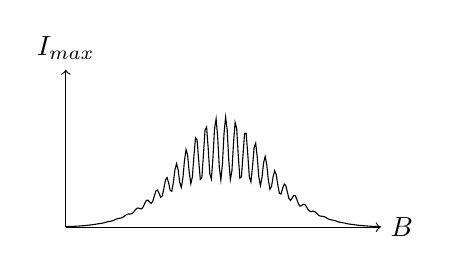
\begin{tikzpicture}[scale=0.2]
                \draw[->] (-10,0) -- (10,0);
                \node[right] at (10,0) {$B$};
                \draw[->] (-10,0) -- (-10,10);
                \node[above] at (-10,10) {$I_{max}$};
                \draw[samples=200, domain=-10:10] plot(\x, {exp(-\x*\x / 10) * 2 * sin(10*deg(\x)) + 5 * exp(-\x*\x / 20)});
                % \draw plot(\x, {sin(\x)});
            \end{tikzpicture}
            \caption{SQUID Data}
            \label{05.11.SQUID}
        \end{figure}
\end{enumerate}

\chapter{19/11/14 --- PC 8 --- The Debye Model}

\section{1D phonon crystal}

We consider a one-dimensional crystal of $N$ equally spaced atoms and want to describe its longitudinal lattice vibrations. We suppose that an elastic force $f_{n, n+1} = -K\left( u_n - u_{n+1} \right)$ acts between neighboring atoms of mass $M$, where $u \ll a$ is the deviation of the atom from equilibrium. The Hamiltonian thus goes
\begin{align}
    H = \sum\limits_{N}^{}\frac{p_n^2}{2M} + \frac{1}{2}M\omega_0^2\left( u_{n+1} - u_n \right)^2
\end{align}
where $\omega_0 = \sqrt{\frac{K}{M}}$. 

We then decompose into Fourier modes, using periodic boundary conditions, so
\begin{align}
    u_n(t) &= \frac{1}{\sqrt{N}}\sum\limits_{q}^{}u_q^2(t)e^{iqna} &
    p_n(t) &= \frac{1}{\sqrt{N}}\sum\limits_{q}^{}p_q^2(t) e^{ipna}
\end{align}
which makes our Hamiltonian
\begin{align}
    H &= \frac{1}{N}\sum\limits_{nqk}^{}\frac{1}{2M}\tilde{p}_q(t) \tilde{p}_k(t)e^{i(k+q)na} + \frac{1}{2}M\omega_0^2 \frac{1}{N}\sum\limits_{nqk}^{}\tilde{u}_q(t) \tilde{u}_k(t)\left[ e^{i(k+q)(n+1)a} - 2e^{i(k+q)na}e^{ikqa} + e^{i(k+q)na} \right]\\
    &= \sum\limits_{q}^{}\frac{1}{2M} \tilde{p}_q(t) \tilde{p}_q(t)(t) + \frac{1}{2}M\omega_0^2\sum\limits_{q}^{}\tilde{u}_p^2(t)u_q^2(t)\left[ 1 - 2e^{-iqa} + 1 \right]
\end{align}
a bunch of poopy algebra that I can't see since the TA is incompetent and writes for ants\dots
\begin{align}
    H &= \sum\limits_{q}^{}\frac{1}{2M}\abs{\tilde{p}_q(t)}^2 + \frac{1}{2}M \sum\limits_{q}^{}\omega_0^2\abs{\tilde{u}_q(t)}^2
\end{align}

We examine the long-wavelength limit $q \to 0$ of $\omega_0$, and we find $\omega_q \to \omega_0 q a$. We define $c_s \equiv \omega_0 a$ the speed of sound, and so $c = \sqrt{\frac{K}{M}}a$ (we often write $c$ instead of $c_s$ when the meaning is clear). Note that this means that sound travels faster in a solid than air since $K$ is larger.

We know that the energy of the total system is given $E = \sum\limits_{q}^{}\left( n_q + \frac{1}{2} \right)\hbar \omega q$. Then by statmech $\expvalue{E} = \sum\limits_{q}^{}\left( \expvalue{n_q} + \frac{1}{2} \right)\hbar \omega_q$ with $\expvalue{n_q}$ given by the appropriate distribution. Since phonos are bosons, we have $\expvalue{n_q} = \frac{1}{e^{\beta\left( \hbar \omega_q \right)} - 1}$.

\section{3D}

Let's go to $3D$. We now represent $\vec{q} = \left( q_1, q_2, q_3 \right)$ with $N$ such vectors. There are $3N$ modes, and there must also be a maximum $q$. In $1D$, $q_{max} = q_{debye} = \frac{2\pi}{a}$. Call then $\lambda$ the polarization of the photon, an index running $1,2,3$, then we compute
\begin{align}
    \expvalue{E} &= \sum\limits_{q,\lambda}^{}\left( \frac{1}{e^{\beta \hbar \omega_{q,\lambda}} - 1} + \frac{1}{2} \right) \hbar \omega_{q,\lambda}\\
    &= \sum\limits_{q,\lambda}^{} \int\limits_{0}^{\infty}d\omega\; \delta(\omega - \omega_{q,\lambda})\left( \frac{1}{e^{\beta \hbar \omega} - 1} + \frac{1}{2} \right)\hbar \omega\\
    &= \int\limits_{0}^{\infty}d\omega\;\left( \frac{1}{e^{\beta \hbar \omega} - 1} + \frac{1}{2} \right)\hbar \omega \sum\limits_{q,\lambda}^{}\delta\left( \omega - \omega_{q,\lambda} \right)\\
    &= \int\limits_{0}^{\infty}d\omega\left( \frac{1}{e^{\beta \hbar \omega} - 1} + \frac{1}{2} \right)\hbar \omega g(\omega)
\end{align}
where we recognize that the summation is just the density of states! 

Then we want the specific heat
\begin{align}
    C = \left( \pd{\expvalue{E}}{T} \right)_{N \nu} &= \pd{\expvalue{E}}{\beta}\pd{\beta}{T}\\
    &= \pd{\expvalue{E}}{\beta}\frac{-1}{k_BT^2} = -k_B \beta^2 \pd{\expvalue{E}}{\beta}\\
    &= \int\limits_{0}^{\infty}d\omega\;\frac{k_B \hbar \omega \beta^2}{\left[ 2\sinh\left( \frac{N\hbar \omega}{2} \right) \right]^2}\hbar \omega g(\omega)\\
    &= k_B \int\limits_{0}^{\infty}\left[ \frac{\hbar \omega \beta}{2 \sinh\left( \frac{\beta \hbar \omega}{2} \right)} \right]^2g(\omega)\;d\omega
\end{align}

We note that in the $\beta \to 0$ limit (the infinite temperature limit) we find $C = 3Nk_B$, the law of Dulong and Petit.

We then ask at low frequencies the density of states. We find
\begin{align}
    g(\omega) &= \sum\limits_{q,\lambda}^{} \delta\left( \omega - \omega_{q,\lambda} \right)\\
    &= 3\sum\limits_{q}^{}\delta\left( \omega - cq \right)\\
    &= 3\int\limits_{}^{}d\vec{q}\;\frac{V}{(2\pi)^3}d^3q\delta\left( \omega - cq \right)\\
    &=\dots\\
    &= \frac{3V\omega^2}{2\pi^2c^3}\Theta(\omega_D - \omega)
\end{align}

We also look into the low temperature $C$, which equates to a large $\beta$, and with some changes of variables and other nonsense we find $C \propto T^3$, and the crux of the math lies in the order of the $\beta$s under the integral. In a different number of dimensions, our derivation of $g(\omega)$ depends on the Jacobian which generally goes like $q^{d-1}$ for $d$ dimensions. So in general $C \propto T^d$.
\chapter{26/11/14 --- PC 9 --- Spin Waves, Magnons}

Consider a chain of atoms with spins that interact, then the Hamiltonian is given
\begin{align}
    H &= -J \sum\limits_{n}^{}\vec{S}_n\vec{S}_{n+1}
\end{align}
such that when spins are aligned energies are minimized and when spins are anti-aligned energies are maximized. For example, at zero temperature a ferromagnet is completely aligned, and increasing the temperature introduces thermalr fluctuations.

\section{Spin waves}
\begin{enumerate}[1.]
    \item \emph{Show the coupling fo a spin to its neighbors can be written as the action of a magnetic field $\vec{B}_n$ acting on $\vec{S}_n$.}
        For such a ferromagnet, we know the Hamiltonian in a magnetic field and the magnetic moment go like
        \begin{align}
            H_n &= -\vec{\mu}_n \cdot \vec{B}_n & \vec{\mu}_n &= \gamma \hbar \vec{S}_n\\
            H_n &= -J \vec{S}_n \cdot \left( \vec{S}_{n+1} + \vec{S}_{n-1} \right) & \vec{B}_n &= \frac{J}{\gamma \hbar}\left( \vec{S}_{n+1} + \vec{S}_{n-1} \right)
        \end{align}
        $\gamma$ the gyromagnetic moment, and we obtain the induced magnetic field as a function of the spins. 

    \item \emph{Show the differential equation that links the dynamics of the spin $S_n$.}
        
        Working the math with his back to the students, the TA finds straightforwardly that
        \begin{align}
            \rd{\vec{L}}{t} &= \tau\\
            \rd{\vec{S}_n}{t} &= \frac{J}{\hbar}\vec{S}_n \times \left( \vec{S}_{n+1} + \vec{S}_{n-1} \right)
        \end{align}
    \item \emph{Denote $\vec{S}_n = S\vec{u}_z + \delta \vec{S}_n$ deviations about the aligned state. Write the llinearized equations.}

        We math like mad, noting that $\rd{S}{t} = 0$ and so defining $\delta \vec{S}_n = \vec{S}_n - S\vec{u}_z = \delta S_n^x(t)\vec{u}_x + \delta S_n^y(t)\vec{u}_y$ we work our way to
        \begin{align}
            \rd{}{t}\delta S_n^x(t) &= -\frac{J}{\hbar}S\left( -2\delta S_n^y \delta S_{n+1}^y + \delta S_{n-1}^y \right)\\
            \rd{}{t}\delta S_n^y(t) &= \frac{J}{\hbar}S\left( -2\delta S_n^x \delta S_{n+1}^x + \delta S_{n-1}^x \right)\\
        \end{align}
        and in general
        \begin{align}
            \rd{(\delta S_n)}{t} &= \frac{iSJ}{\hbar} \left( -2 \delta S_n + \delta S_{n+1} + \delta S_{n-1} \right)
        \end{align}

    \item \emph{Decouple these little mofos.}

        Maaaaaaaaaaaaaaaaaaaath. We write into eigenmode decompositions
        \begin{align}
            \delta S_n &= \frac{1}{\sqrt{N}} \sum\limits_{k}^{}S_K e^{i(kna - \omega_kt)}
        \end{align}
        and plugging through the equations above, doing the typical bash for such problems (recall finite coupled harmonic oscillators from Ph12a) we obtain the familiar dispersion relation
        \begin{align}
            \omega_k &= \frac{4SJ}{\hbar}\sin^2 \frac{ka}{2}
        \end{align}

    \item \emph{How does the dispersion behave at small $k$? Why does a spin wave carry a mass?}

        In the $k \to 0$ limit, $\omega_k \sim \frac{SJk^2a^2}{\hbar}$ for small $\sin$ approximation. Thus, we can rewrite this into $\hbar \omega_k = Ak^2, A = SJa^2$, but also associated with $\hbar \omega_k$ is a momentum $\frac{\hbar^2 k^2}{2m^*}$ and so we can associate with the spin wave a mass
        \begin{align}
            m^* &= \frac{\hbar^2}{2SJa^2}
        \end{align}

    \item \emph{Find the total magnetization and energy in the limit of small deviations.}

        Continuing to talk to the board and to block all vision of equations, we compute the magnitude of the magnetization
        \begin{align}
            \vec{S}_n &= S_n' \hat{u}_z + \delta \vec{S}_n\\
            \abs{\vec{S}_n}^2 &= S_n'^2 + \abs{\delta \vec{S}_n}^2 = S^2\\
            \abs{\delta \vec{S}_n}^2 &= \delta \vec{S}_n \cdot \delta \vec{S}_n = \delta S_n \delta S_n^* = \abs{\delta S_n}^2
            \mu_z &= \gamma \hbar \sum\limits_{n}^{}\sqrt{S^2 - \abs{\delta S_n}^2}\\
            &\dots
            &= \gamma \hbar \left( NS - \frac{1}{2S}\sum\limits_{K}^{}\abs{S_k}^2 \right)
        \end{align}

        Then to find the energy we just plug and chug
        \begin{align}
            E &= -J \sum\limits_{n}^{}S_n' S_{n+1}' - J\sum\limits_{n}^{}\delta \vec{S}_n \cdot \delta \vec{S}_{n+1}\\
            &\dots
            &= -NJS^2 + \frac{1}{2S}\sum\limits_{K}^{}\abs{S_k}^2 \hbar \omega_k
        \end{align}
\end{enumerate}

\section{Quantification of spin waves, magnons}

Quantification of magnons proceeds just like for phonons (thankfully, Edward Perpelinsky also discussed that petite classe). Their energy is $E = \hbar \omega_k$ and their occupation number is given by the Bose-Einstein distribution (magnons are like photons/phonons and are thus bosons, or you can have multiple magnons in a given mode)
\begin{align}
    n_k &= \frac{1}{\exp\left( \frac{\hbar \omega_k}{k_BT} \right) - 1}
\end{align}

The mean energy of bosons in general is given
\begin{align}
    E(T) &= -NJS^2 + \sum\limits_{k}^{}n_k \hbar \omega_k
\end{align}
which comparing with our above expression yields
\begin{align}
    \mu_z &= \gamma \hbar\left( NS - \sum\limits_{K}^{}n_k \right)
\end{align}

\section{Thermodynamics of spin waves, 3D}

Place the atoms in a 3D lattice now instead. We assume that for long wavelength excitations the dispersion relation is still given by the above.

\begin{enumerate}[1.]
    \item \emph{Compute the internal energy/magnetization at a finite temperature $T$.}

        We simply replace the sum from the previous part with an integral and we obtain
        \begin{align}
            E &= -NJS^2 + \int\limits_{0}^{\infty}d\omega\;n(\omega)\hbar \omega g(\omega)\\
            \mu_z &= \int\limits_{0}^{\infty}d\omega\;\gamma \hbar n(\omega) g(\omega)
        \end{align}

    \item \emph{Calculate the density of states of the spin waves in three dimensions.}

        We compute
        \begin{align}
            g(\omega) &= V\int\limits_{}^{}\frac{d^3k}{(2\pi)^3}\;\delta\left( \omega - Ak^2 \right)\\
            \delta\left( \omega - Ak^2 \right) &= \frac{\delta\left( k - \sqrt{\frac{\omega}{A}} \right)}{2A\sqrt{\frac{\omega}{A}}} + \frac{\delta\left( k + \sqrt{\frac{\omega}{A}} \right)}{2A\sqrt{\frac{\omega}{A}}}\\
            &= \frac{\delta\left( k - \sqrt{\frac{\omega}{A}} \right)}{2\sqrt{\frac{\omega}{A}}}
        \end{align}
        where we throw out the second delta function since it's not within the bounds of integration. Continuing
        \begin{align}
            g(\omega) &= \frac{Na^3}{2\pi^2}\frac{1}{2A\sqrt{\frac{\omega}{A}}}\int\limits_{}^{}k^2 \delta\left( k - \sqrt{\frac{\omega}{A}} \right)\;dk\\
            &= \frac{Na^3}{4\pi^2}\frac{1}{A}\sqrt{\frac{\omega}{A}}
        \end{align}

    \item \emph{Calculate the relative variation of the magnetization at low temperature.}

        Denote $\mu_{z,0}$ the zero temperature magnetization. Then we do some really hard work and we find
        \begin{align}
            \frac{\Delta \mu_z}{\mu_{z,0}} &= \frac{0.059}{S}\left( \frac{k_BT}{SJ} \right)^{3/2}
        \end{align}
        which is \emph{Bloch's Law}.

    \item \emph{Calculate the specific heat at low temperatures.}

        Blah dee blah blah, we obtain
        \begin{align}
            C_v &= 0.113 N k_B \left( \frac{k_BT}{JS} \right)^{3/2}
        \end{align}

    \item \emph{What about multiple dimensions?}

        The big change going to multiple dimensions is the density of states, as usual. Again, the Jacobian changes to $k^{D-1}$ in $D$ dimensions, and since each $k$ contributes an $\omega^{1/2}$, and we find dependencies
        \begin{align}
            \Delta \mu_z \propto T^{\frac{D}{2}}
            C_v \propto T^{\frac{D}{2}}
        \end{align}
\end{enumerate}

\end{document}
